

\section{Presentación del proyecto}
El proyecto aquí detallado permitirá a toda persona la unificación y centralización de la totalidad de su información relacionada con el bienestar y salud, poniéndola a disposición de la misma o de terceros autorizados.

Proporcionará el ingreso de distintos tipos de datos y estudios que serán gestionados personalmente, presentando un medio de uso simple, ágil e intuitivo para alentar y facilitar su uso.
Uno de los objetivos es que la persona pueda hacer uso de esta aplicación desde cualquier lugar del mundo y en cualquier momento, a través de Internet, usando un dispositivo móvil o una PC.

Brindará al propietario de la información, la posibilidad  de interactuar con los profesionales médicos de su preferencia, brindándole a ellos los permisos adecuados para realizar consultas, seguimientos, aportar comentarios y/o dar conclusiones según sus requerimientos.

El proyecto estará dirigido por los lineamientos del software libre, para lo cual no sólo se hará uso de tecnologías textit{open source}, sino que también estará públicamente disponible.


\section{Relevamiento general}

\subsection{Relevamiento de la organización}

Actualmente puede observarse que en forma generalizada, tanto en nuestra provincia, país y mayormente en todo el mundo, los hospitales y organizaciones de salud manejan la información del paciente mediante historias clínicas dentro de la misma institución en forma privada, limitando el acceso del paciente a la misma.
Esto plantea una idea falsa de la universalidad de la información, ya que si una persona se hace atender en un centro médico, tendrá los datos de los estudios que se ha realizado en ese lugar; sin embargo, no tendrá acceso a los que pudo haberse realizado en otras instituciones en el pasado, ni podrá brindar toda esta información a los futuros centros médicos a los que asista.

En el mundo se ha comenzado a fomentar la idea de una historia clínica universal, e incluso hay lugares en los cuales se exige a los centros médicos que hagan uso de un sistema centralizada de  información.
El problema es que sigue siendo una idea o punto de vista centrado en los centros médicos y no en la personas.

Hoy en día existen aplicaciones que brindan una solución parcial al problema antes mencionado, pero no permiten al usuario el control y disposición en forma completa de su información, ya que carecen de la posibilidad de hacer uso de los mismos libremente (por ejemplo, al poder compartirla con profesionales médicos de su preferencia), de migrar sus datos a los sistemas que consideren oportunos, y de manejar la privacidad de la información sin tener que aceptar obligatoriamente los términos y condiciones de empresas que lucren o se reserven derechos sobre éstos.

Este proyecto tiene por objetivo resolver las falencias detectadas en el contexto mundial actual, permitiendo que el control de la historia clínica pase a manos de la persona, propietaria real de los datos.


\subsection{Relevamiento de las funciones detectadas}
En este apartado se presentarán los conceptos básicos de Carpeta de Salud Personal, se expondrá el contexto actual utilizando como ejemplo el Hospital Italiano de Mendoza, haciendo hincapié en todo lo referido a historia clínica del mismo y se informará sobre aquellas herramientas existentes en el mercado que son similares al proyecto que se pretende desarrollar.

\subsection{Registro médico electrónico}
	Antes de hacer una introducción de las herramientas que se encuentran en el mismo campo de acción vamos a pasar por los conceptos que forman sus cimientos.
Lo primero que debemos hacer es establecer la diferencia entre \textbf{registro médico electrónico} (Electronic Medical Record - EMR) y \textbf{sistema de información de salud}. El EMR es solo un componente de un SIS. Su función es la adquisición, almacenamiento, recuperación, procesamiento e intercambio de datos clínicos relacionados a un paciente. Los \textbf{datos clínicos}, hacen referencia a distintos aspectos de la información de un paciente..hábitos, problemas médicos, antecedentes familiares, examen físico, resultados de exámenes complementarios, etc. Estos son creados y usados por médicos, enfermeras, especialistas, como así también por otros profesionales de la salud. Para cerrar el concepto de RME dejamos la definición que hace de la misma este proyecto que plantea una iniciativa open health, \textbf{Good European Health Record} (GEHR), el registro médico debe ser una colección de datos y hechos registrados en forma manuscrita, gráficamente o en formato electrónico, como medio para preservar el conocimiento. Debe ser un diario de información de datos clínicos, registrados en un tiempo y lugar, por un profesional de la salud. Esto debería estar accesible en todo momento y lugar, por profesionales autorizados, y debería poder ser compartido entre diferentes sistemas. Debemos distinguir dos conceptos fundamentales, el \textbf{EMR} y el \textbf{Registro de Salud Electrónico} (Electronic Health Record - EHR), el primero es el que está circunscrito a una sola institución y el segundo integra toda la información de un paciente más allá de una sola institución

\subsubsection{Carpeta de salud}
Una \textbf{Carpeta de Salud}, según lo visto en la sección anterior, cae dentro de los que es un \textbf{EHR} y es una herramienta de gestión y archivo de la información de salud que es mantenida por el paciente.
Esto contrasta con la Historia Clínica tradicionalmente proporcionada y gestionada por las instituciones sanitarias,
como los hospitales o servicios públicos de salud,
y contiene información introducida por profesionales sanitarios o de gestión relacionada con los servicios proporcionados por entidades aseguradoras.

El objetivo de una \textit{Carpeta de Salud} es proporcionar un resumen completo y correcto del historial médico de un individuo, y que éste sea accesible online.
Una Carpeta de Salud puede incluir información sobre pruebas diagnósticas, analíticas, informes de médicos y terapeutas,
 variables de salud introducidas por el paciente o recogidas de forma automática por dispositivos electrónicos de medida.
Algunos de los beneficios que se le atribuyen a una Carpeta de Salud son:
	\begin{itemize}
        \item Mejora de la capacidad de autogestión de los pacientes.
	    \item Posibilidad de implantación de planes de salud pública o de comunicación de información de utilidad para pacientes.
	    \item Alta personalización de los tratamientos, rehabilitaciones y planes de seguimiento para cada paciente.
	    \item Reducción de errores derivados de la intervención de distintos profesionales sobre un mismo paciente, como por ejemplo en la prescripción de medicación.
	    \item Mejoras en la calidad percibida de los servicios derivada de una relación médico-paciente basada en una comunicación más constante a través de Internet.
	\end{itemize}


\subsubsection{Historia clínica electrónica}
%veo si lo dejo así o como historia clínica electrónica ambulatoria

Según Institute of Medicine, IOM, una historia clínica electrónica, HCE, es aquella que reside en un sistema electrónico específicamente diseñando para recolectar, almacenar, manipular y dar soporte a los usuarios en cuanto a proveer accesibilidad a datos seguros y completos, alertas, recordatorios y sistemas clínicos de soporte para la toma de decisiones, brindando información clínica importante para el cuidado de los pacientes, la cual es ampliada con los siguientes conceptos:
	\begin{itemize}
    \item Colección longitudinal de información electrónica sobre la salud de las personas, donde la información es definida como “información pertinente a la salud de un individuo provista por un profesional sanitario”.
    \item Acceso electrónico inmediato a la información de salud personal o poblacional solamente de usuarios autorizados.
    \item Provisión de bases de conocimiento y sistemas de soporte para la toma de decisiones que mejore la calidad, seguridad y eficiencia de la atención de los pacientes.
    \item Soporte efectivo en la eficiencia de los procesos para brindar cuidados de salud.
    \end{itemize}
   A partir de esta definición vemos que HCE es mucho más que solo un EMR, podemos verla como una integración de múltiples sistemas existentes, en primera medida podríamos dividirlo en dos sistemas componentes: 
	\begin{itemize}
    	\item Información específica del paciente: se genera durante la atención de los mismos.
        \item Información basada en el conocimiento: está contenida en la literatura científica o
los fundamentos científicos de las ciencias de la salud.
	\end{itemize}
    La HCE como otros sistemas de EHR surge en respuesta a los problemas que planteaba el uso en papel, organización, cantidades\/volúmenes de información, incompletitud, accesibilidad, falta de seguridad, redundancia, investigación, calidad, reutilización, legibilidad, etc aportando los siguientes beneficios:
    \begin{itemize}
		\item Accesibilidad y disponibilidad de los datos del paciente.
		\item Múltiples visualizaciones de los datos.
		\item Comunicación con otros profesionales.
		\item Comunicación con los pacientes.
		\item Agregación de datos. (resúmenes y agrupación de los datos)
        \begin{itemize}
			\item Medición de calidad del desempeño médico
			\item Identificación rápida de casos
		\end{itemize}
		\item Acceso a bases de conocimientos.Información contextual como edad, sexo, raza, problemas, tratamientos que recibe, factores de riesgo, etc.
		\item Integración con soporte para la toma de decisiones.
	\end{itemize}
Tenemos distintas formas de clasificar el EMR según como se organice la información:
\begin{itemize}
	\item Orden cronológico
	\item Centrado en el paciente
	\item Orientación a nivel de atención
	\item Registro ordenado por fuentes
	\item Orientación a problemas
	\item Orientación a especialidades
	\item Orientación a patologías
\end{itemize}
En el caso de la orientación a nivel de atención se nos presentan dos modalidades de atención:
\begin{itemize}
	\item Registros longitudinales: abarcan toda la vida del individuo, desde su nacimiento hasta su muerte. En el ámbito ambulatorio, el registro es continuo al igual que la atención y está representado por la historia clínica ambulatoria
    \item Registros episódicos: son registros que mantienen un episodio fijo de salud. Se caracterizan por tener una fecha de comienzo y una de final bien acotada. Pueden finalizar con un resumen de los cuidados realizados que sirve como medio de comunicación entre los profesionales (epicrisis). Están representados por historia clínica de internación, historia clínica de medicina domiciliaria y historia clínica de emergencias/guardia.
\end{itemize}


\subsubsection{Health Vault}
	 Es una aplicación gratuita con soporte web y móvil en el que una persona puede reunir, almacenar, usar y compartir su propia información personal de salud, y las de los miembros de su familia. Brindando una API para la conexión con distintos tipos de dispositivos y aplicaciones móviles, Microsoft Health Vault deja las puertas abiertas a posibilidades ilimitadas. 
     Debemos tener en cuenta de que se trata de un producto enlatado y web por lo que las funciones relevadas son las que podemos observar simplemente registrándonos, esto no implica que el sistema por detrás tenga mas funcionalidades de soporte para el nivel estratégico.
     
     Sin embargo es una aplicación que no esta totalmente disponible para Argentina, ya que no se puede descargar la aplicación para nuestro dispositivo móvil, retringiendonos muchas funcionalidades relacionadas a los distintos tipos de carga de datos.
     Aunque el sistema estuviera disponible en nuestro país, no cuenta con la posibilidad de adjuntar documentos a patologías del paciente, a mediciones, o a tratamientos registrados, lo que convierte la gestión de documentos en simplemente una carpeta online, privando al usuario de verificar todos los documentos correspondientes a un tratamiento de forma fácil. Para realizar esa carga el sistema de Microsoft provee de una herramienta adicional llamada Microsoft Connection Center siendo una complejidad adicional la necesidad de su instalación además de ser un software que solo funciona bajo los sistemas operativos Microsoft Windows.
	
    Entre otras funcionalidades limitadas que hemos notado, se encuentra el hecho de que el sistema no permite la carga de información por parte del Médico para el paciente, si no es solo a través del sistema Direct, el cual esta solo disponible para EEUU, por lo que consideramos que es necesario un sistema alternativo que posibilite su carga de otra manera.
    
	Además el sistema no tiene un seguimiento particular sobre las embarazadas siendo un grupo de riesgo y considerado de mucho interés para nuestro sistema porque implica la incorporación de dos nuevos usuarios(la madre y el hijo).
     
\subsection{Situación legal del país}   
La Ley 26.529 establece los derechos del paciente referido a la documentación e información clínica y a la relación con los profesionales e instituciones de salud. 

En el apéndice \ref{Ley-26.529} se puede observar los artículos mas importantes de la ley extraída de la página oficial del ministerio de salud del gobierno de la provincia de Bs As.




\subsection{Tecnología de la información}
 A continuación se detallan la infraestructura y las técnologías de los Hospitales que hacen uso de una historia clínica centralizada
 Data center con una sala de servidores, sala de energía (UPS y generadores), central telefónica, diseñado cumpliendo normas, 80 servidores de datos, capacidad de almacenamiento en línea de 400TB, redes que soportan telefonía, datos y multimedia, servidores de aplicaciones, de base de datos y balanceo de carga.
 Ver \textbf{Figura \ref{infgen}}.
 
\begin{sidewaysfigure}
  \centering
  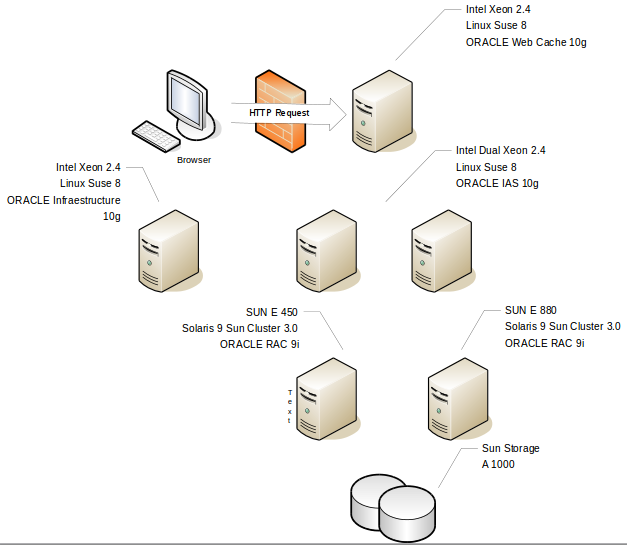
\includegraphics[width=.8\textwidth]{img/tp1/modeloGrande}
  \caption{Infraestructura general}
  \label{infgen}
\end{sidewaysfigure}

    \textbf{Arquitectura}: Servidor central de mensajería 
    
\textbf{HL7:}
 que se comunica con los demás sistemas de laboratorio, farmacia, diagnóstico por imagen, facturación e HCE, el sistema de HCE presenta una interfaz web que permite el acceso y brinda funcionalidades diferentes a médicos, administradores y pacientes. Ver \textbf{Figura \ref{esthl7}}.
\begin{figure}
  \centering
  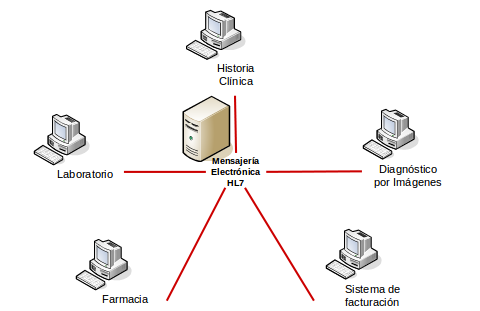
\includegraphics[width=.8\textwidth]{img/tp1/hl7}
  \caption{Estándar HL7}
  \label{esthl7}
\end{figure}

	\textbf{Software}: componentes que forman la arquitectura del software desarrollado por el hospital. Ver \textbf{Figura \ref{arqsw}}.
\begin{figure}
  \centering
  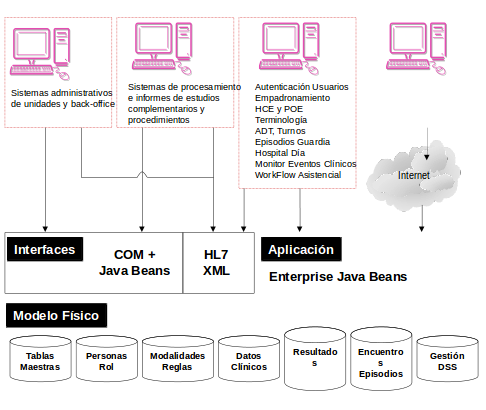
\includegraphics[width=.8\textwidth]{img/tp1/modgenfinal}
  \caption{Arquitectura del software}
  \label{arqsw}
\end{figure}

Al relevar Health Vault encontramos que se ha usado un esquema orientado a los servicios, a través de una interfaz basada en XML para una mayor independencia del backend, y así permitir que desarrolladores ajenos a la empresa puedan hacer uso de estos servicios y colaborar de alguna manera con su proyecto. Además utilizan un servidor web IIS corriendo sobre un plataforma Microsoft Windows Server y el proyecto fue desarrollado en ASP.NET apoyándose sobre algunos frameworks para la vista como JQuery, JQueryUI y KnockoutJS.

{\correccionTexto
\subsubsection{Estándares}
En cuanto a tecnologías de información nos pareció indispensable relevar los distintos estándares que se usan en los registros médicos y de cuidado de la salud, dentro de estos encontramos:

\begin{enumerate}
	\item\textbf{HL7 v3} es conjunto de especificaciones de interoperabilidad para transacciones entre sistemas de información y aplicaciones de software utilizados en el sector salud, que forma parte del conjunto de estándares HL7. Características:
    	\begin{itemize}
			\item Cuenta con un Modelo de Referencia de Información
            \item Contempla el uso de sintaxis XML
            \item Utiliza principios de Orientación a Objetos (POO) y Lenguaje de Modelado Unificado (UML)
            \item No se limita a la capa 7 del modelo OSI
            \item Hace un fuerte énfasis en el uso de vocabularios controlados
		\end{itemize}
    %Fuente: https://es.wikipedia.org/wiki/HL7_v3
    
    \item\textbf{CIE10}  Clasificación internacional de enfermedades, décima versión correspondiente a la versión en español de la ICD. Determina la clasificación y codificación de las enfermedades y una amplia variedad de signos, síntomas, hallazgos anormales, denuncias, circunstancias sociales y causas externas de daños y/o enfermedad. Cada afección puede ser asignada a una categoría y recibir un código de hasta seis caracteres de longitud en formato de X00.00. Cada una de estas categorías puede incluir un grupo de enfermedades similares.
    %Fuente: https://es.wikipedia.org/wiki/CIE-10
    
    \item\textbf{SNOMED-CT} nomenclatura de medicina sistematizada \- términos clínicos. Es la terminología clínica integral, multiling\"{u}e y codificada de mayor amplitud, precisión e importancia desarrollada en el mundo.
    %Fuente: https://es.wikipedia.org/wiki/Snomed-CT
    
    \item\textbf{ATC} Sistema de clasificación anatómica, terapéutica y química, define un índice de sustancias farmacológicas y medicamentos, organizados según grupos terapéuticos. Este sistema fue instituido por la Organización Mundial de la Salud, y ha sido adoptado en Europa. El código recoge el sistema u órgano sobre el que actúa, el efecto farmacológico, las indicaciones terapéuticas y la estructura química del fármaco. Representa una categorización estructurada en 5 niveles.
    %Fuente: https://es.wikipedia.org/wiki/C%C3%B3digo_ATC
    
    \item\textbf{CDA} Arquitectura de documento clínico. Es un estandar de lenguaje de marcado basado en XML con el objetivo de especificar la codificación\/cotejamiento, estructura y semantica de documentos clínicos para su intercambio. CDA especifíca la sintaxis y provee un framework para especificar la semántica completa de un documento clínico. Define a este documento como aquel que tiene las siguientes 6 características:
      \begin{itemize}
          \item Persistencia
          \item Administración
          \item Potencial de autenticación
          \item Contexto
    	  \item Integridad
   		  \item Legibilidad humana
      \end{itemize}
      %Fuente: https://en.wikipedia.org/wiki/Clinical_Document_Architecture
      
    \item\textbf{CIAP-2} Clasificación internacional de atención primaria. Es una taxonomía de los términos y expresiones utilizadas habitualmente en medicina general\/de familia. Recoge los motivos (o razones) de consulta, los problemas de salud y el proceso de atención. Es un tipo de clasificación de terminología médica de ámbito internacional. La clasificación CIAP-2 contiene 17 capítulos, diferenciados por una letra que corresponden a un código nemotécnico en inglés.
    %Fuente: https://es.wikipedia.org/wiki/Clasificaci%C3%B3n_Internacional_de_Atenci%C3%B3n_Primaria
    
    \item\textbf{CPOE} Registro computarizado de órdenes para medicina, es un proceso en el cuál el médico registra instrucciones para el tratamiento del paciente (particularmente para pacientes hospitalizados) bajo su cuidado. Estas órdenes son comunicadas a través de redes de computadora al equipo médico o los departamentos (farmacia, laboratorio, radiología entre otros) responsables de ejecutar lo establecido en la orden. CPOE reduce el retraso al completar la orden, reduce los errores relacionados con la escritura a mano o traducción, permite el ingreso de ordenes en el punto de cuidado (centro médico) o fuera del mismo, provee chequeo de errores para dosis o pruebas duplicadas o incorrectas y simplifica el inventario y publicación.
    %Fuente: https://en.wikipedia.org/wiki/Computerized_physician_order_entry
    
    \item\textbf{CCR} Continuidad del registro de cuidado, referido también como CRC, estándar definido por ASTM (American Society for Testing Materials), es un estándar para el registro del resumen médico de pacientes. Es una forma de crear documentos flexibles que contienen la información más relevante e importante, por el factor tiempo, sobre un paciente. Este es enviado electrónicamente de un responsable médico a otro. Contiene varias secciones tales como datos demográficos, datos sobre seguros médicos, diagnostico, problemas, medicaciones, alergias y planes de cuidados médicos. Representan una "imagen" del estado de un paciente que puede resultar útil en el momento de un encuentro clínico.
    %Fuente: https://es.wikipedia.org/wiki/Continuidad_del_Registro_del_Cuidado
    
    
    \item\textbf{CCD}
	Este artefacto especificado por HL7 es una guía de implementación provista para el intercambio de registros de atención continua por parte de los pacientes.Esta basado en las características estipuladas por CDA aplicadas a CRR. De esta manera CDD establece un amplio conjunto de plantillas que representan las secciones típicas los registros médicos y expresa estas plantillas en base a las restricciones impuestas por CDA. Estas plantillas pueden ser para signos vitales, historia familiar,plan de atención,entre otros aspectos. 
    
    \item\textbf{OpenEHR} Comunidad virtual trabajando en interoperabilidad y computabilidad en salud electrónica (e-health) su foco principal son sistemas EHR (Electronic Health Records). La fundación ha publicado un conjunto de especificaciones definiendo un modelo de referencia en información médica, un lenguaje para construir ``modelos clínicos'', o arquetipos, que son separados del software y un lenguaje de consulta. La arquitectura está diseñada para hacer uso de terminologías de salud externa como SNOMED-CT, LOINC y ICDx. 
    %Fuente: http://www.openehr.org/home
    
\end{enumerate}
}

% \section{Relevamiento General}
% \subsection{ Relevamiento de la Organización}
% \textit{EXPLICACION: Motivación o la iniciativa que dio lugar a la idea del proyecto (estado actual del mundo...)}
% \subsection{ Relevamiento de las funciones detectadas e interfaces.}
% \textit{Especificar los dos relevamientos detectados: un lugar específico de la provincia (estado actual en el país), y las herramientas encontradas que realizan funciones similares.}
% \subsection{Tecnología de la información.}
% \textit{Tecnologías con lo que está hecho / utiliza el hospital y los sistemas competidores (ejemplo: servidores del hospital, sistemas web, ...)}
% \section{Relevamiento Detallado}
% \subsection{ Detalle, explicación y documentación detallada de todas las funciones seleccionadas.}
% \section{ Diagnóstico de la situación actual}
% \subsection{Modelo lógico del Sistema actual.}
% \subsection{ Problemas y necesidades detectados en las funciones relevadas en detalle y en su entorno organizacional.}
% \subsection{Objetivos y alcances preliminares del nuevo Sistema. OBJETIVOS DEL SISTEMA:}

\clearpage
\section{Relevamiento Detallado}
Este apartado pretende describir aquellas aplicaciones ya existentes en el mercado que hacen uso de la Carpeta Médica Personal, de un modo similar a la idea que pretendemos llevar a cabo en el presente proyecto.


\subsection{Microsoft Health Vault}
	 Es una aplicación gratuita con soporte web y móvil en el que una persona puede reunir, almacenar, usar y compartir su propia información personal de salud, y las de los miembros de su familia. Se trata de un producto enlatado y web por lo que las funciones relevadas son las que podemos observar simplemente registrándonos.
     Esto no implica que el sistema por detrás tenga más funcionalidades de soporte para algún nivel estratégico.
{\correccionTexto	
\subsubsection{Procesos}
A continuación se detallarán los procesos que se encuentran representado en el diagrama de Flujo de datos de la \textbf{Figura \ref{hv_data_flow}}
}
	\begin{correccionFigure}[h]
      \centering
      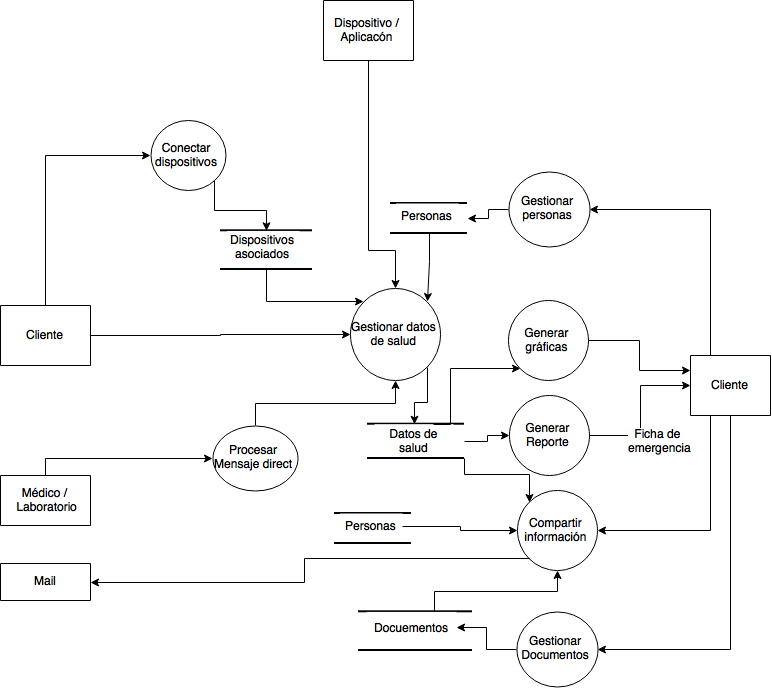
\includegraphics[width=.8\textwidth]{img/tp1/hv_flujo_de_datos}
      \caption{Diagrama de flujo de datos, de Health Vault.}
      \label{hv_data_flow}
    \end{correccionFigure} 


\begin{itemize}
 {\correccionTexto
\item \textbf{Gestión de datos referidos a la salud}
	El sistema permite registrar diferentes tipos de datos médicos y personales donde se cargan desde cuestiones básicas como el peso o la altura hasta las más complejas como la composición corporal o la glucosa, véase \textbf{Figura \ref{carga_peso} y Figura \ref{carga_comidas}}.  Permitiendo entre otras cosas:
    \begin{itemize}
		\item \textbf{Registrar todos los detalles}, tanto si desea administrar problemas graves de salud como si desea comprobar el bienestar de su familia. Esto permite realizar un seguimiento detallado de todo tipo de características relacionadas a la salud.
        \item \textbf{Realizar un seguimiento de los valores cargados} para controlar las afecciones crónicas mediante los dispositivos conectados que facilitan la carga de datos. El seguimiento de los valores permiten observar las tendencias, descubrir patrones, proporcionar datos más completos a los médicos y conservar la motivación para tomar mejores decisiones con respecto a la salud.
        \item \textbf{Acceso a los datos} siempre que exista una conexión a internet.
	\end{itemize}
 
 	\begin{correccionFigure}[h]
      \centering
      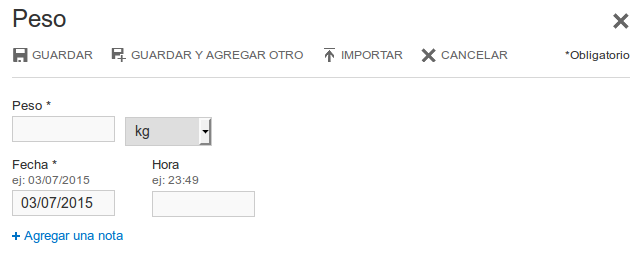
\includegraphics[width=.8\textwidth]{img/tp1/3-carga_peso}
      \caption{Formulario de carga del peso}
      \label{carga_peso}
    \end{correccionFigure}   
    
	\begin{correccionFigure}[h]
      \centering
      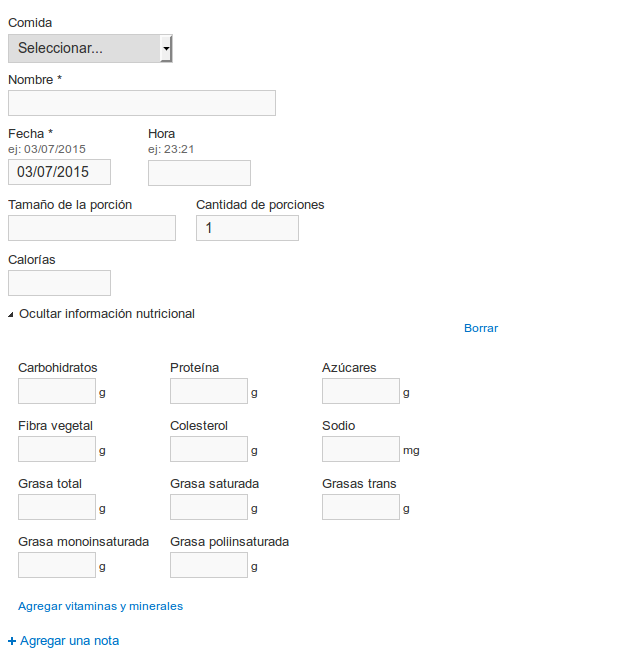
\includegraphics[width=.8\textwidth]{img/tp1/3-carga_comidas}
      \caption{Formulario de carga de comidas y bebidas}
      \label{carga_comidas}
    \end{correccionFigure} 
    }
\clearpage
 {\correccionTexto
\item \textbf{Gestión de los miembros del grupo familiar}, este es un aspecto bastante natural y necesario en los PHR, ya que en muchos casos un miembro del grupo familiar, gestiona información del resto, como es en el caso de los padres sobre los hijos. El sistema le permite conserve todos los registros médicos propios y de la familia en un solo lugar, donde estén ordenados y disponibles en línea ver \textbf{Figura \ref{carga_miembro}}. 

	\begin{correccionFigure}[h]
      \centering
      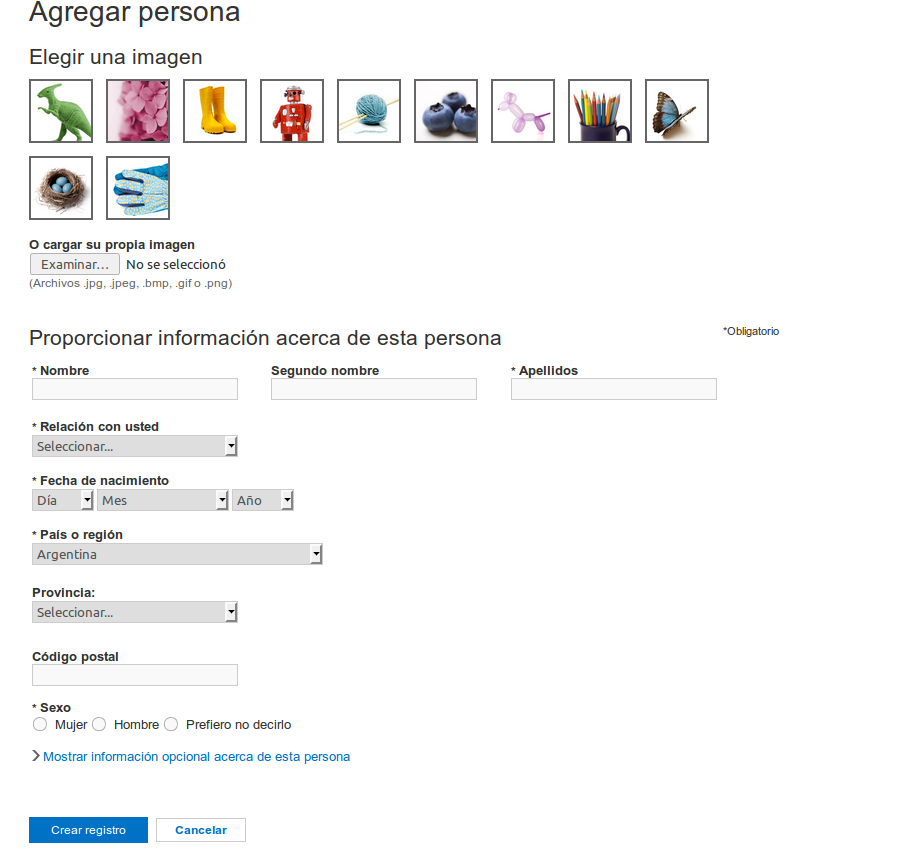
\includegraphics[width=.8\textwidth]{img/tp1/3-carga_miembro}
      \caption{Formulario de carga de un miembro del grupo familiar}
      \label{carga_miembro}
    \end{correccionFigure} 
    
\item \textbf{Carga de documentos},podemos cargar diferentes tipos de archivos multimedia como videos, imágenes y sonido, ver \textbf{Figura \ref{carga_documento}}. 
También desde la web podemos guardar arhivos XML que cumplan con el estandar CCR o CCD (ambos fueron explicados en la sección anterior).

Si necesitaramos cargar algun tipo de estudio especifico de imágenes médicas(de formatos especificos y mayor tamaño) se debe realizar a través de Microsoft Connection Center,una aplicación de escritorio para Windows. Como un punto flaco, Health Vault, no nos permite asociar los documentos a otra información que ya tengamos en el sistema, simplemente podemos adjuntarle una nota.

	Debemos destacar que el sistema permite a las organizaciones, los doctores y los pacientes enviar información de salud cifrada directamente a los destinatarios a través de Direct. 
    Siendo el médico el encargado de cargar la información (Aunque el servicio de Direct está disponible solamente para EE.UU.).%FIXME, sería importante explicar un poco mas direct, en la sección de tecnología de info(2.5)
}	
    \begin{correccionFigure}[h]
      \centering
      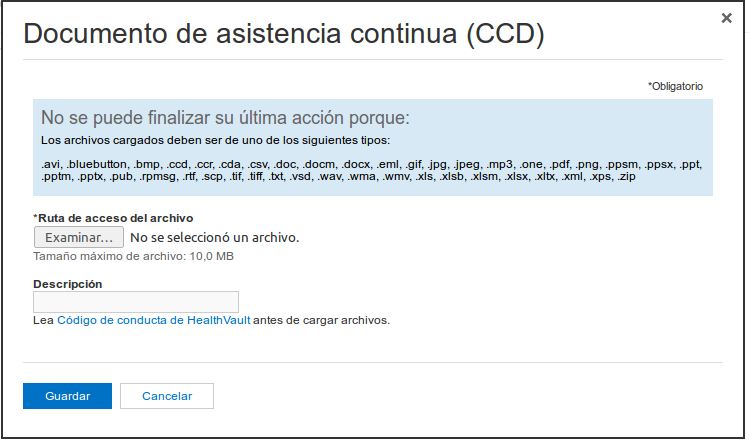
\includegraphics[width=.8\textwidth]{img/tp1/3-carga_documento}
      \caption{Formulario de carga de un documento de salud}
      \label{carga_documento}
    \end{correccionFigure} 
 {\correccionTexto
\item \textbf{Generación de reportes}, el sistema ofrece la posibilidad de generar una ficha de emergencia  con información básica y esencial sobre el paciente para de este modo poder organizar y proporcionar este tipo de información al médico. Permite entre otras cosas:
	\begin{itemize}
		\item Obtener gráficas de los cambios históricos en ciertas mediciones registradas; como por ejemplo, peso, medidas corporales, comidas, entre otros, vea \textbf{Figura \ref{graficas}}.
        \item Obtener listas actualizadas de alergias y medicamentos
		\item Obtener lecturas recientes obtenidas en asistencia domiciliaria (como presión arterial, glucosa y peso)
		\item Obtener historial de salud
        \item Obtener los cambios realizados a lo largo de un período determinado, en la \textbf{Figura \ref{lista_de_cambios}} se puede ver la vista para seleccionar que registros  consultar .
        \item Generar tarjetas de bolsillos con código de especial que permite el acceso a los datos personales, ver \textbf{Figura \ref{tarjeta_bolsillo}}.
	\end{itemize}
    
    \begin{correccionFigure}[h]
      \centering
      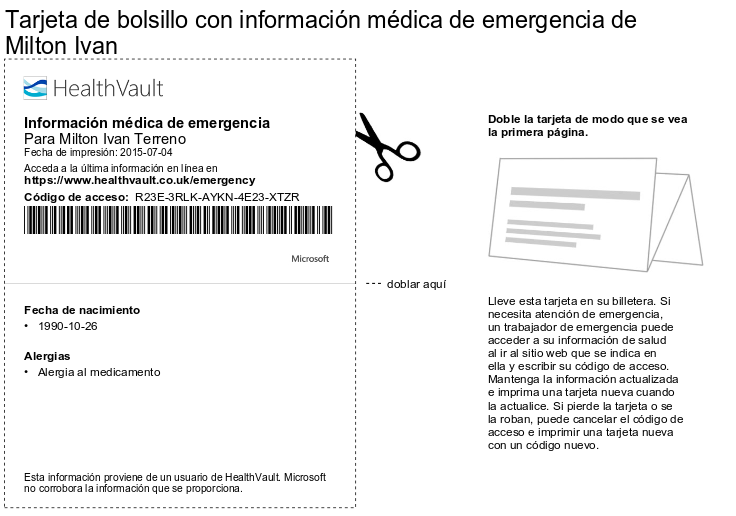
\includegraphics[width=.8\textwidth]{img/tp1/3-tarjeta_bolsillo}
      \caption{Tarjeta de bolsillo}
      \label{tarjeta_bolsillo}
    \end{correccionFigure} 
    
    \begin{correccionFigure}[h]
      \centering
      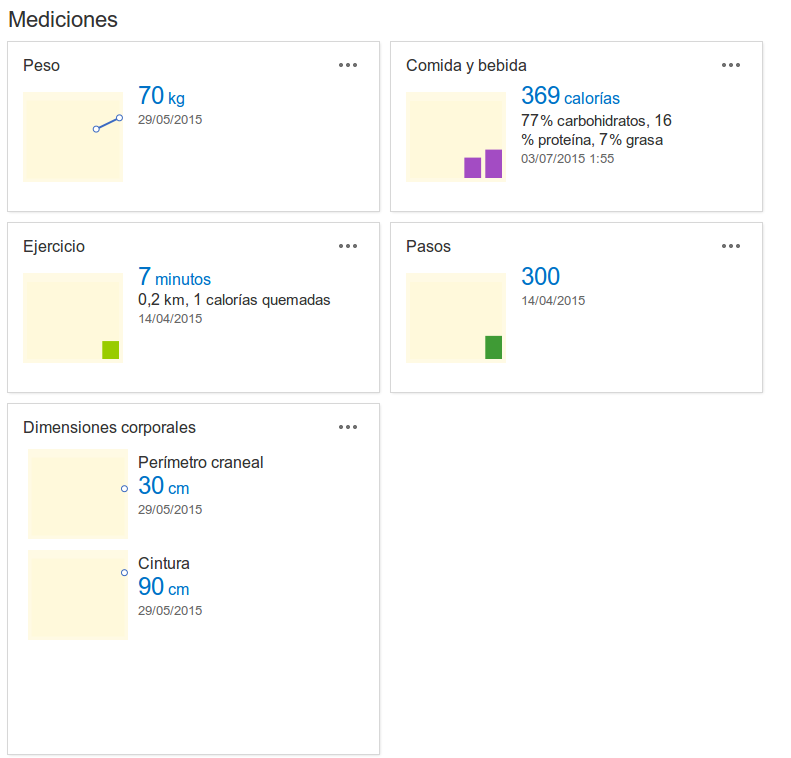
\includegraphics[width=.8\textwidth]{img/tp1/3-graficas}
      \caption{Distintas gráficas ofrecidas por la plataforma}
      \label{graficas}
    \end{correccionFigure} 
    
    \begin{correccionFigure}[h]
      \centering
      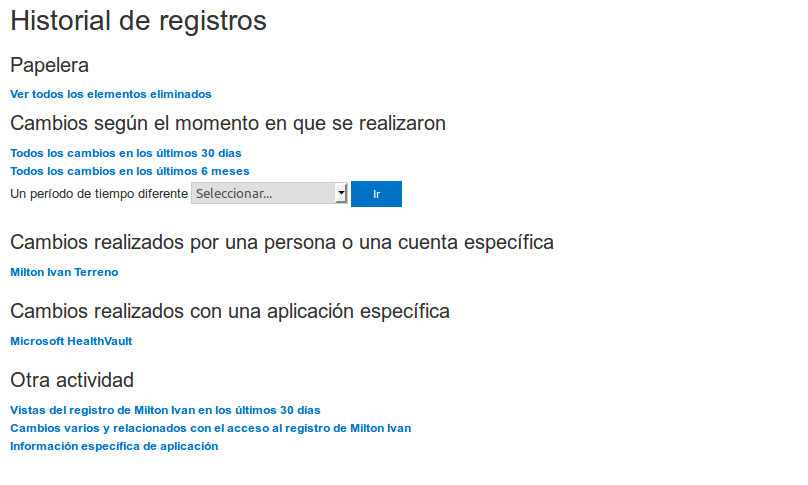
\includegraphics[width=.8\textwidth]{img/tp1/3-lista_de_cambios}
      \caption{Historial de registros}
      \label{lista_de_cambios}
    \end{correccionFigure} 
  
\item \textbf{Conectarse con otras aplicaciones}, Health Vault nos ofrece una API basada en XML, para poder conectarse con diferentes tipos de dispositivos electrónicos, ya sean wearables,smartphones o específicos de algún aspecto de salud (vease \textbf{Figura \ref{conexion_con_dispositivos}}). Para esto ofrece un panel donde podemos ver los dispositivos asociados a la cuenta . 

Esto es importante para realizar un seguimiento sobre determinadas actividades físicas, o sobre aspectos de la salud donde es necesaria su medición continua. Conociendo estos valor podremos realizar modificaciones con fundamentos para aumentar la eficacia de nuestros esfuerzos y nuestra calidad de vida.

    \begin{correccionFigure}[h]
      \centering
      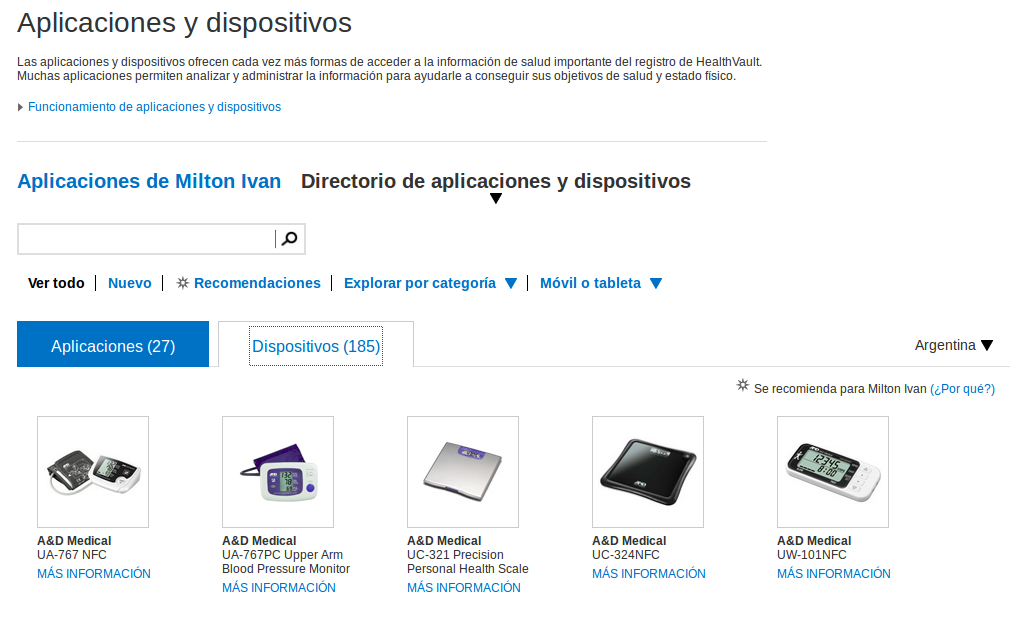
\includegraphics[width=.8\textwidth]{img/tp1/3-conexion_con_dispositivo}
      \caption{Selección de dispositivo}
      \label{conexion_con_dispositivos}
    \end{correccionFigure} 

\item \textbf{Compartir información de salud}
	Se puede compartir información personal, a través de un correo que se envía desde la plataforma de Health Vault, donde previamente se debe seleccionar la información que se desea enviar así como el correo del destinatario y una fecha de caducidad (de los datos enviados), luego el destinatario recibe un link, que para mostrarle la información le exige tener una cuenta en Health Vault. La ficha que se debe llenar para permitir la compartición de archivos con otros usuarios se puede ver en la \textbf{Figura \ref{compartir_perfil}}
    
    El sistema permite entre otras cosas:
    \begin{itemize}
		\item Permite establecer objetivos compartir en las redes sociales nuestra evolución con respecto a ello.
        \item Permite cambiar el tipo de acceso a diferentes datos
%		\item No posee una sección de médicos o alguna forma de interacción con ellos (salvo la de carga de información). 

	\end{itemize}
	\begin{correccionFigure} 
      \centering
      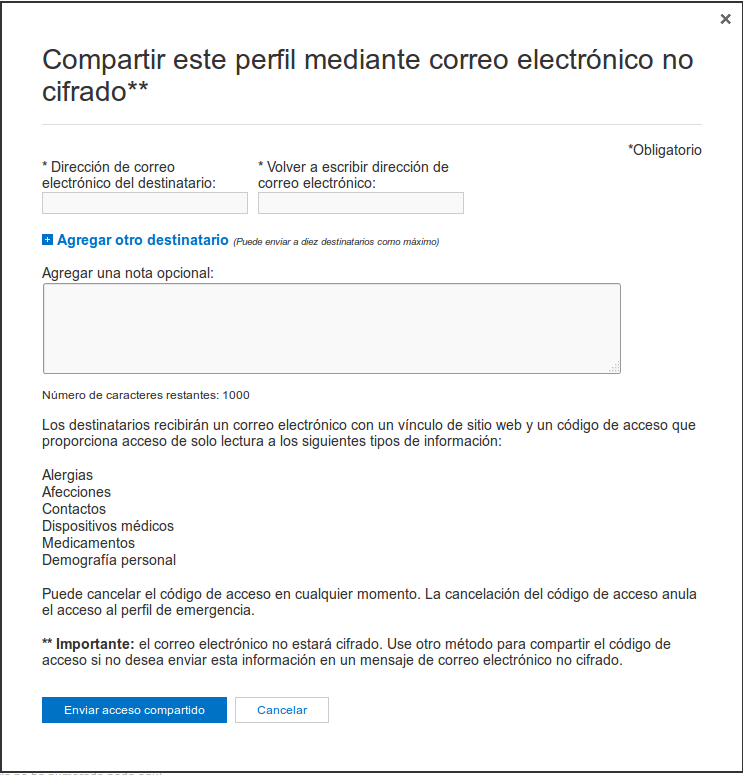
\includegraphics[width=.8\textwidth]{img/tp1/3-compartir_perfil}
      \caption{Formulario para la compartición de archivos}
      \label{compartir_perfil}
    \end{correccionFigure} 
    
    \begin{correccionFigure}[h]
      \centering
      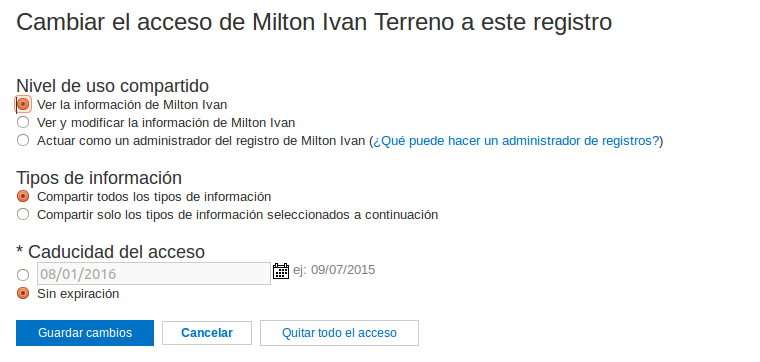
\includegraphics[width=.8\textwidth]{img/tp1/3-cambiar_permisos}
      \caption{Edición de los permisos de acceso a la información}
      \label{cambiar_permisos}
    \end{correccionFigure} 
}  
\clearpage
\subsubsection{Plataforma}

En la actualidad se ofrece soporte para IOS y Android , aunque no permite la carga de archivos por este medio.

	Desde el punto de vista de factibilidad debemos tener en cuenta que no estamos hablando de un software pensado para nuestra país, ya que al acceder desde un dispositivo Android (que tiene la mayor cuota de mercado)  nos informa que el servicio no esta disponible para Argentina. 
	
	Además el hecho de necesitar un software que sólo funciona sobre Windows como Microsoft Connection Center se convierte en una limitación para los usuarios que no pueden acceder a tal Sistema Operativo, y como dijimos anteriormente, sería sumamente interesante que el servicio para la gestión de archivos se brindara para otra plataforma, sobre todo alguna móvil.
\end{itemize}



\clearpage
\subsection{Historia clínica electrónica}

{\correccionTexto
\subsection{Introducción}
Nuestro proyecto posee funcionalidades con características muy relacionadas a lo que conocemos como sistema de Historia Clínica ampliamente utilizado por los hospitales del mundo, estudiando profundamente los distintos tipos de PHR (Registro Personal de Salud) electrónicos nos encontramos con que estos sistemas pueden ser totalmente independientes o estar interconectados con sistemas de historia clínica. Como consideramos la posibilidad de que nuestro proyecto escale el sistema entonces tendría que poder comunicarse con este tipo de sistemas lo que hace la relación aún más fuerte. Por otro lado, lo que diferencia y separa estos sistemas es la disposición de la información en base a quién es el usuario final, los PHR se interesan en como presentar la información a personas no idóneas en el campo de la medicina mientras que la Historia Clínica busca la mejor forma de presentar la información a un médico o persona instruida en medicina. Sin tener en cuenta esta diferencia y ponderando la estrecha relación entre estos sistemas es que hemos decidido relevar un sistema de información de Historia Clínica, en este caso particular, el sistema de Historia Clínica del Hospital Español de Mendoza.
Primero vamos a listar las funcionalidades básicas que debe cubrir un sistema que lleve el historial médico de una persona, luego nos introduciremos de lleno en la aplicación.
}

\subsection{Listado de funciones básicas}

\subsubsection{Gestión de información de salud}
Gestión de problemas actuales y pasados del paciente, gestión de medicamentos, registro de alergias, profesionales que intervinieron al paciente, gestión de evolución clínica en términos narrativo o plantillas estructuradas.

\subsubsection{Gestión de resultados}
Presentación de resultados de estudio en los distintos formatos posibles, texto, imagen, serie de imágenes, interfaces con los distintos proveedores internos que permiten la carga en la historia clínica electrónica de estos resultados.

\subsubsection{Gestión de ordenes médicas}
Gestión de pedidos de estudios de laboratorios, radiológicos, pedidos de farmacia, pedido de estudio anátomo patólogo entre otros. 

\subsubsection{Soporte a la toma de decisiones}
Presentación de la información del paciente que permite al profesional de salud tomar decisiones con la mayor cantidad de información posible. Alertas o recordatorios sobre potenciales problemas o recomendaciones.

\subsubsection{Sistemas de comunicación electrónica y conectividad}
Además de recibir información de servicios auxiliares externos y de otros sistemas a través de mensajería estándar y con terminología consensuada, permite la comunicación entre colegas y con interfaces usadas con el cliente.

\subsubsection{Soporte al paciente}
Envía información al paciente sobre condiciones de salud, tests diagnósticos o tratamientos, lo que mejora la relación médico-paciente y la educación del paciente.

\subsubsection{Procesos administrativos}
Interconexión con sistemas que realizan estadísticas de interés para investigaciones médicas.

\subsubsection{Reporte y salud pública}
Soporte para reporte de bases de datos nacionales de forma automática.

\subsection{Relevamiento sistema Historia Clínica}
A continuación se detalla el relevamiento de la Historia Clínica del Hospital Español de Mendoza.

{\correccionTexto
\subsubsection{Introducción}
La historia clínica a sido desarrollado como un sistema web,  utilizando el framework openerp que brinda una api para desarrollar módulos y extender módulos previamente desarrollados, la aplicación corre en un servidor del hospital, esta presenta una dirección url para ser accedida desde un navegador en cualquiera de las computadoras conectadas a la intranet del hospital. Las tecnologías usadas para el desarrollo son:

\begin{itemize}
	\item\textbf{Lenguaje de programación:} Python
    \item\textbf{Base de datos:} PostgreSQL
    \item\textbf{Plantillas FrontEnd:} Werkzeug
    \item\textbf{Vistas del lado del servidor:} Qweb
    \item\textbf{Reportes:} JasperReports
\end{itemize}

\subsubsection{Login}
Desde cualquier navegador podemos escribir la url y se nos presentará la siguiente vista para el login. \textbf{Figura \ref{login-sistema}}
Cada paciente, médico, auditor médico, director médico poseen un usuario y contraseña para acceder al sistema
}

\begin{correccionFigure}[h]
      \centering
      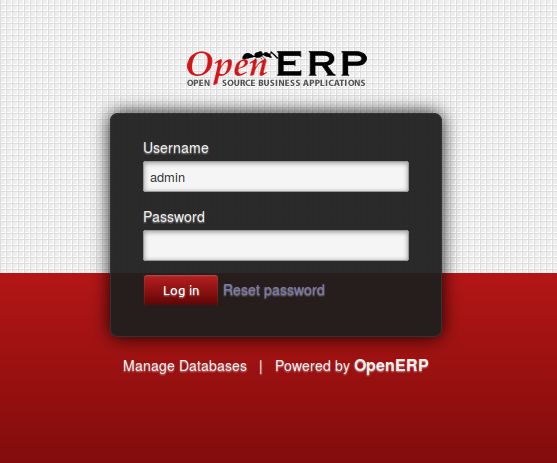
\includegraphics[width=.8\textwidth]{img/tp1/HE/Login}
      \caption{Login}
      \label{login-sistema}
\end{correccionFigure} 

{\correccionTexto
\subsubsection{Pantalla principal}
Una vez que ingresemos al sistema, como muestra la \textbf{figura \ref{pantalla-princip}}, se nos presenta una pantalla en la cual la barra superior contiene los nombres de módulos de acuerdo al perfil que se ha asignado al usuario logeado, una barra lateral izquierda que presenta los menúes para el módulo en el que nos encontramos actualmente, en la parte superior derecha nos muestra el nombre de usuario con el que ingresamos y en la parte superior izquierda la compañía a la que pertenece el sistema.
}

\begin{correccionFigure}[h]
      \centering
      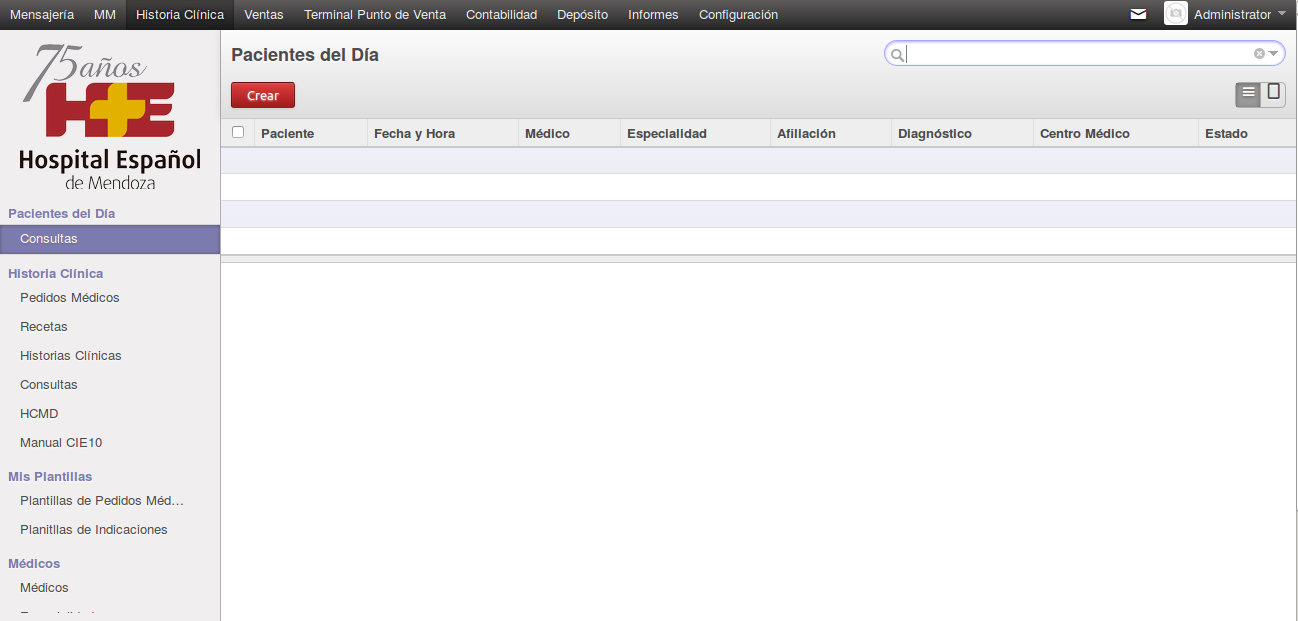
\includegraphics[width=.8\textwidth]{img/tp1/HE/PantallaPrincip}
      \caption{Pantalla principal}
      \label{pantalla-princip}
\end{correccionFigure}

{\correccionTexto
\subsubsection{Módulo Historia Clínica}
Para entrar al sistema de Historia Clínica seleccionamos el módulo con el nombre correspondiente y se nos muestran los menúes Pacientes del día con su submenú Consultas, el menú central Historia Clínica, submenúes Pedidos Médicos, Recetas, Historias Clínicas, Consultas, Historia Clínica Manual Digital, Manual CIE10, el menú Mis Plantillas, submenúes Plantillas de Pedidos Médicos y Plantillas de Indicaciones, menú Médicos con submenúes Médicos y Especialidades, el menú Informes con submenú Prácticas y el menú Configuración con submenú Tipo de Atención. La siguiente \textbf{Figura \ref{submenu}} muestra los menúes presentes en el módulo.
}

\begin{correccionFigure}[h]
      \centering
      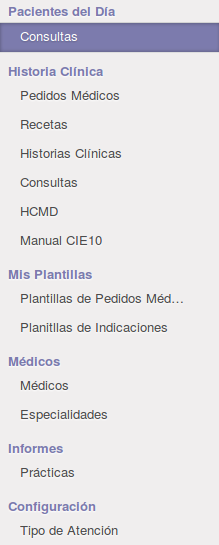
\includegraphics[height=.3\textheight]{img/tp1/HE/MenuHC}
      \caption{Menues}
      \label{submenu}
\end{correccionFigure}

{\correccionTexto
\subsubsection{Consultas del día}
Apenas ingresamos al módulo de Historia Clínica lo primero que nos muestra es la lista de Consultas que el médico asociado al usuario actual tiene asignadas para atender en el corriente día, esta lista presenta columnas para filtrar las consultas por nombre y apellido del paciente, fecha de consulta, nombre del médico, su especialidad, afiliación, diagnóstico, centro médico y estado de la consulta.
Si damos al botón Crear el sistema nos muestra el formulario para crear la consulta, este formulario presenta el número de consulta y requiere el ingreso de la fecha y hora, nos presenta 3 pestañas: Principal, Adjuntos y Examen físico. 
La pestaña de adjuntos es para adjuntar cualquier tipo de archivo, pdf, planilla de texto, planilla de cálculo, imágenes entre otros.
La pestaña de examen físico presenta un cuadro de texto libre para que el médico cargue todas las observaciones que crea pertinente durante la consulta.
En la pestaña principal podemos ver los datos del paciente, su nombre, edad, la Institución con la cuál a contratado un seguro de salud y su número de afiliado en la institución. Muestra también los datos del médico, su nombre y especialidad la cual puede ser seleccionada en un nomenclador previamente configurado por un administrador con las posibles especialidades que puede tener un médico, ofrece un cuadro de texto para que el médico pueda escribir el motivo de la consulta de forma libre, presenta una sección para que el médico pueda determinar el diagnóstico usando un nomenclador que tiene precargado por el administrador la clasificación establecida por el CIE10, además se provee un botón con un enlace al manual online para su consulta, como otra sección se presentan los tratamientos, los pedidos médicos para que la persona realice estudios médicos (imágenes, análisis clínicos entre otros), las recetas para los medicamentos que debería consumir el paciente en su proceso de recuperación y las indicaciones que debe seguir para la mejora. Como las indicaciones pueden repetirse se brinda un nomenclador de plantillas para que el médico seleccione las plantillas de indicaciones que alla armado previamente. En la parte superior de la consulta podemos ver los estados por los que puede pasar la consulta, una vez creada queda en espera, cuando la persona esta siendo atendida por el médico pasa a estado en consultorio y cuando finaliza la atención pasa a finalizada. En cualquier momento la consulta puede ser cancelada dejando establecido explícitamente el motivo.\textbf{Figura \ref{consulta-dia}}}

\begin{correccionFigure}[h]
      \centering
      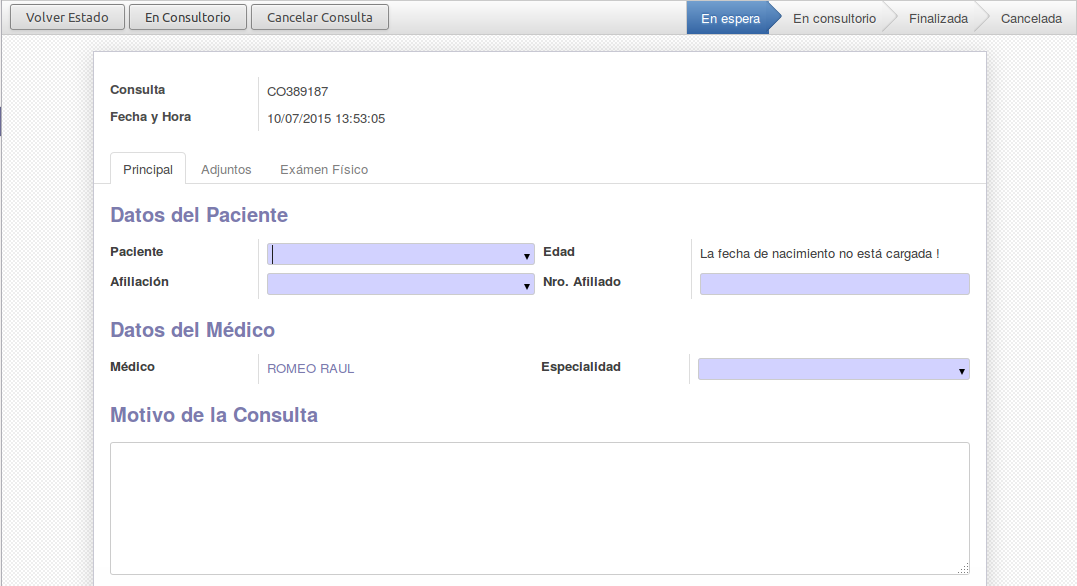
\includegraphics[width=.8\textwidth]{img/tp1/HE/ConsultaDia}
      \caption{Consultas}
      \label{consulta-dia}
\end{correccionFigure}

{\correccionTexto
\subsubsection{Pedidos médicos}
Entrando al submenú Pedidos Médicos del menú de Historia clínica podemos ver listados los Pedidos Médicos realizados por el médico asociado al usuario, este listado puede ser filtrado por el nombre del paciente para ver el histórico de pedidos médicos realizado por el médico para un paciente específico. Los pedidos médicos son las solicitudes de estudios médicos que arman los especialistas para sus pacientes, entre los diferentes estudios médicos encontramos estudios de laboratorios, anatomías patológicas, análisis clínicos, imágenes. Los pedidos generalmente son disparados desde la consulta. En el listado podemos ver una serie de columnas con los datos del pedido, datos que podemos usar para ordenar la lista, en este caso podemos ordenar la lista por paciente, fecha y hora, médico prescriptor, especialidad, afiliación, diagnóstico para cuyo caso se presenta un nomenclador que siempre trae los códigos más usados por el médico, centro médico (ya que el hospital presenta tres sucursales médicas) y tipo de atención (si es ambulatoria o Internado). Al crear un pedido médicos se debe cargar los datos del paciente, nombre y apellido, edad, afiliación, número de afiliado, médico prescriptor, especialidad del médico, tipo de atención, fecha y hora del pedido, diagnóstico y el detalle del pedido indicando los estudios que pueden ser cargados a partir de una plantilla previamente cargada. Una vez finalizada la carga, el pedido se imprime, se firmado por el médico y el paciente lo usa como comprobante para hacerse el estudio en el hospital. \textbf{Figura \ref{pedido-medico}}}

\begin{correccionFigure}[h]
      \centering
      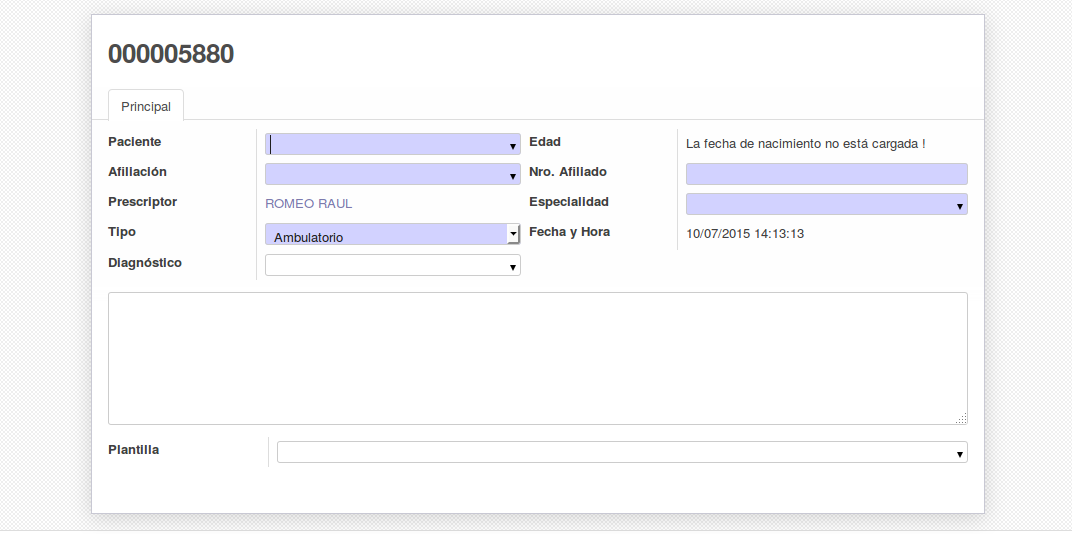
\includegraphics[width=.8\textwidth]{img/tp1/HE/PedidoMedico}
      \caption{Pedido médico}
      \label{pedido-medico}
\end{correccionFigure}

{\correccionTexto
\subsubsection{Recetas}
En este submenú el médico puede ver el listado de todas las recetas generadas por el médico asociado al usuario activo, el listado muestra los datos correspondientes a las columnas nombre y apellido del paciente, fecha registro de la receta, médico prescriptor, especialidad de este último, afiliación, diagnóstico, centro médico y tipo de atención. Al cargar una nueva receta el médico carga los datos del paciente como en el caso del pedido médico, cabe aclarar que al cargar el nombre del paciente se carga automáticamente otros datos relacionados y se filtran algunos de los nomencladores. Para la receta específicamente el médico indica primero la monodroga del medicamento, luego al seleccionar la presentación se filtra en el nomenclador solo las presentaciones conformadas por esa monodroga y por último el médico indica la cantidad de envases que debe comprar el paciente, se deja también un cuadro de texto libre para que el médico indique las observaciones que sean pertinentes.\textbf{Figura \ref{receta}}}

\begin{correccionFigure}
      \centering
      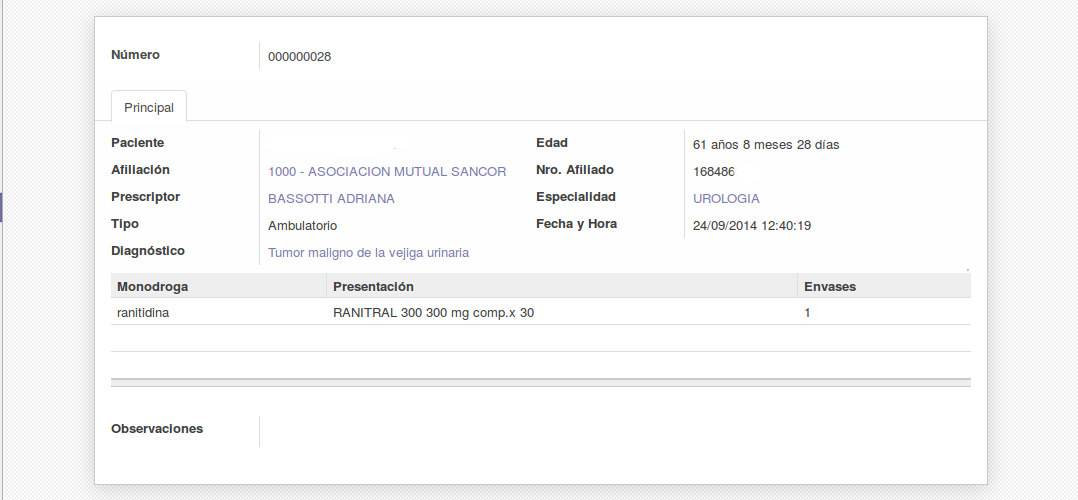
\includegraphics[width=.8\textwidth]{img/tp1/HE/Receta}
      \caption{Carga de receta}
      \label{receta}
\end{correccionFigure}

{\correccionTexto
\subsubsection{Prácticas}
Muestra al médico las practicas que ha solicitado a un paciente a través de un pedido médico, selecciona una práctica y tomando como referencia los resultados de la práctica, elabora un informe y establece un diagnóstico.
\textbf{Figura \ref{practica-medica}}}

\begin{correccionFigure}
      \centering
      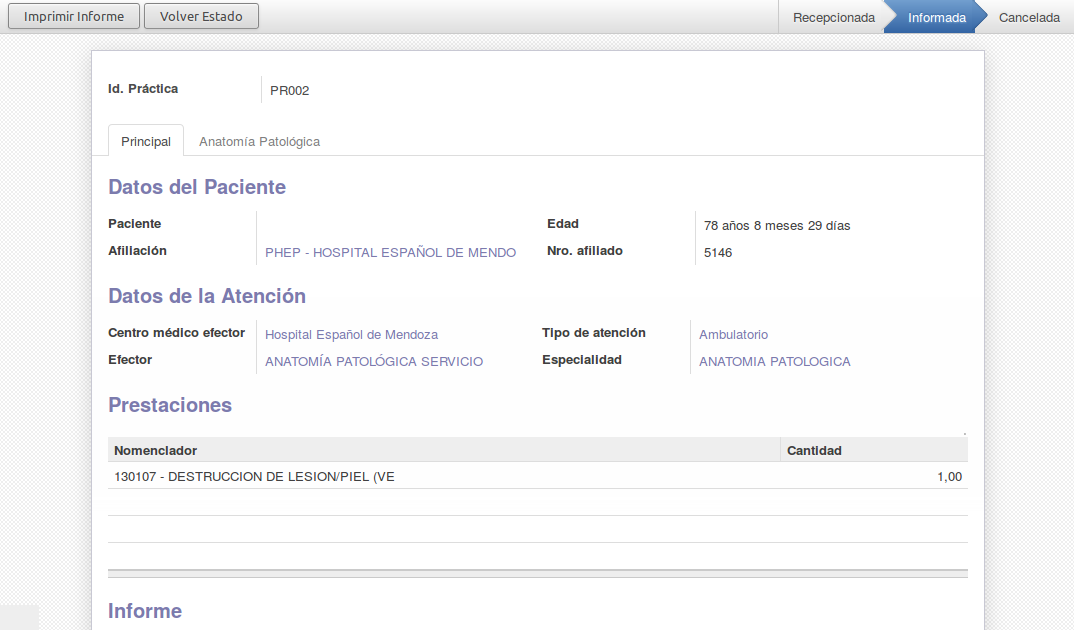
\includegraphics[width=.8\textwidth]{img/tp1/HE/Practica1}
      \caption{Ejemplo práctica}
      \label{practica-medica}
\end{correccionFigure}

{\correccionTexto
\subsubsection{HC manual digitalizada}
A través del submenú HCMD el sistema nos muestra el listado de todas las historias clínicas manuales que han sido digitalizadas en el hospital, si seleccionamos para observar una en particular nos encontramos con que tenemos la imagen de la historia clínica manual, la ruta en la que se encuentra la imagen en el filesystem del servidor que las almacena y las observaciones que se hayan cargado al momento de la digitalización.
Ocurre que en algunos consultorios no poseen el equipamiento hardware necesario por lo que la historia clínica sigue haciendose en papel entonces es útil esta funcionalidad para digitalizar las imágenes.\textbf{Figura \ref{HCMD}}}

\begin{correccionFigure}[ht]
      \centering
      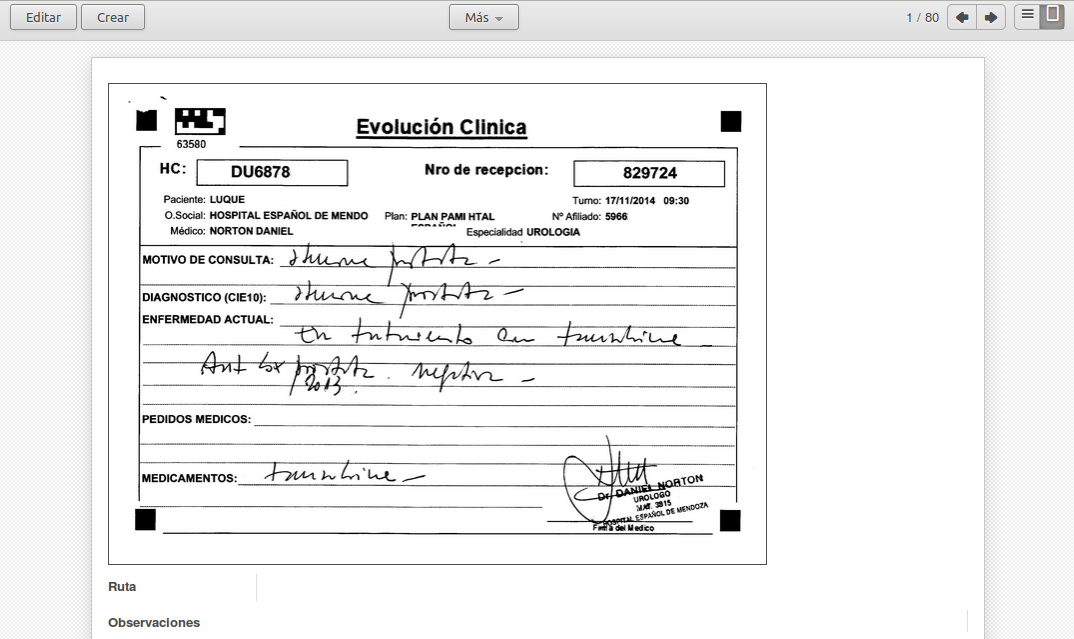
\includegraphics[width=.8\textwidth]{img/tp1/HE/HCMDmanualdigital}
      \caption{Historia clínica manual digitalizada}
      \label{HCMD}
\end{correccionFigure}

{\correccionTexto
\subsubsection{Historia clínica}
Este es el submenú que utiliza generalmente el médico y presenta el camino común de uso del sistema por parte del médico. Al ingresar a este submenú lo primero que ve el médico es listado de los pacientes cuya historia clínica el médico asociado al usuario tiene permisos para consultar.
Si le damos al botón crear nos encontramos con un formulario de alta de historia clínica para un paciente, este formulario presenta como campos obligatorios (aquellos cuadros de texto que vemos con fondo gris) el nombre y apellido el paciente, el tipo y número de documento y el sexo, otros datos opcionales son la fecha de nacimiento, edad, grupo sanguineo y estado civil. Se puede cargar los datos para contactar al paciente, dirección, teléfono fijo, celular, fax, email y sitio web. Cuando le damos a guardar queda iniciada la historia clínica del paciente.
Volviendo a la vista que presenta el listado de pacientes, vemos que muestra otros detalles como una imagen del paciente, su número de historia clínica, edad y sexo. El médico generalmente desde esta vista seleccionará el paciente y pasará a una vista donde
En la parte superior de esta vista vemos una serie de botones, estos nos llevan a las vista de lista de por ejemplo las consultas previas, este botón nos mostrará la lista de consultas previas del paciente asociadas a su historia clínica, así también, con los otros botones podemos ver sus prácticas, internaciones previas, imágenes tomadas, laboratorios, pedidos médicos, recetas e historias clínicas manuales digitalizadas. En este menú y haciendo uso de los botones indicados previamente el médico puede consultar toda la información histórica necesaria para una mejor toma de decisiones. 
Cabe destacar de los botones mencionados el botón de imágenes, este botón nos conecta con una aplicación corriendo en un servidor del hospital usada para ver las imágenes que se han tomado en el hospital pasando el id (documento) del paciente para que filtre las imágenes del mismo. Las imágenes que se muestran siguen el estándar Dicom. Las figuras de la carga de historia clínica y el software de imágenes pueden verse en la \textbf{Figura \ref{hc-principal}} y la \textbf{Figura \ref{sw-imagen}}}

\begin{correccionFigure}[h]
      \centering
      \begin{subfigure}[t]{0.48\textwidth}
        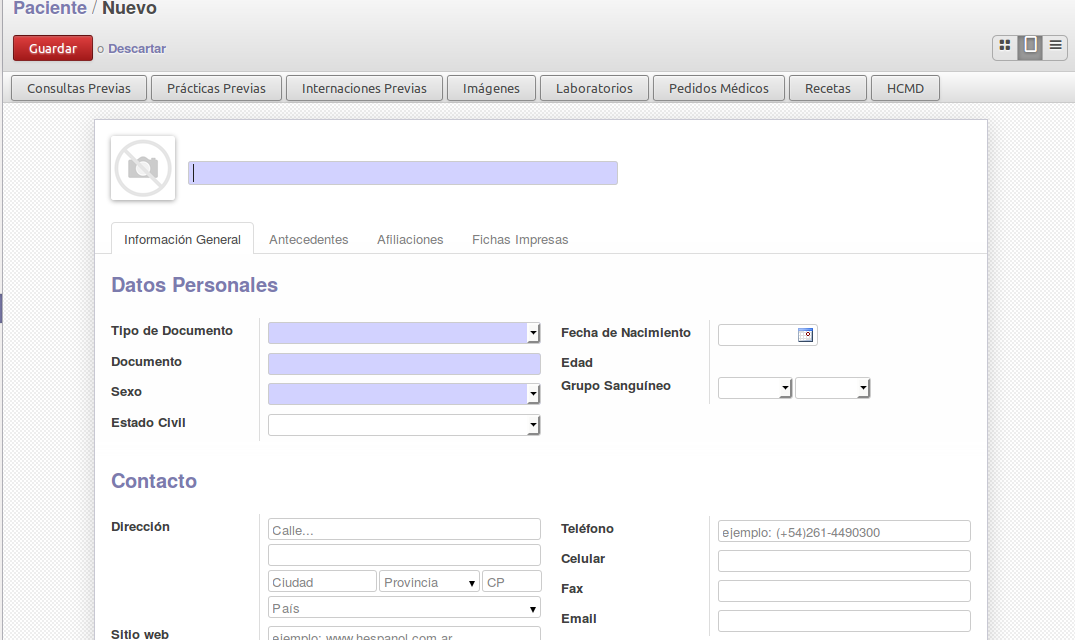
\includegraphics[height=3.5cm]{img/tp1/HE/HCUD2}
        \caption{Crear historia clínica}
        \label{hc-nueva}
      \end{subfigure}
      \hfill%
      \begin{subfigure}[t]{0.548\textwidth}
        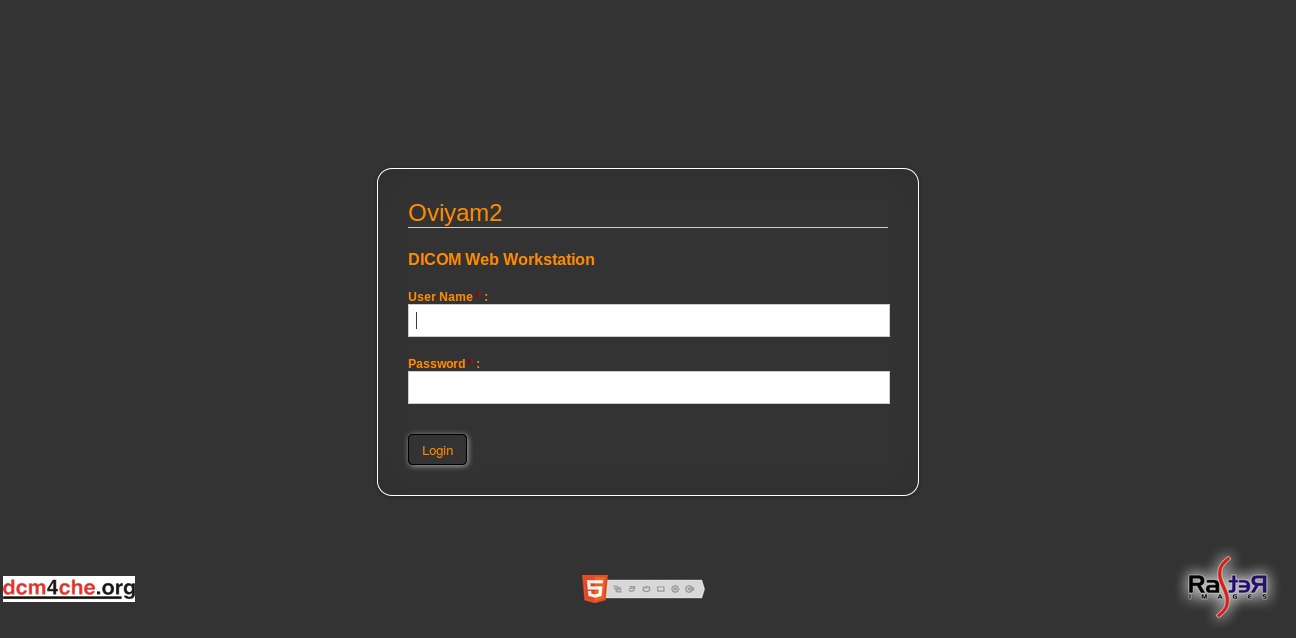
\includegraphics[height=3.5cm]{img/tp1/HE/Imagenes}
        \caption{Software para imágenes}
        \label{sw-imagen}
	  \end{subfigure}
\end{correccionFigure}

{\correccionTexto
\subsubsection{Auditor}
Hay botones como el de consulta, recetas y prácticas que son usados por los auditores del hospital para controlar la actividad realizada por todos los médicos del hospital, este es un listado que no puede ver un médico por su perfil. \textbf{Figura \ref{consultas-auditor}}
}

\begin{correccionFigure}[h]
      \centering
      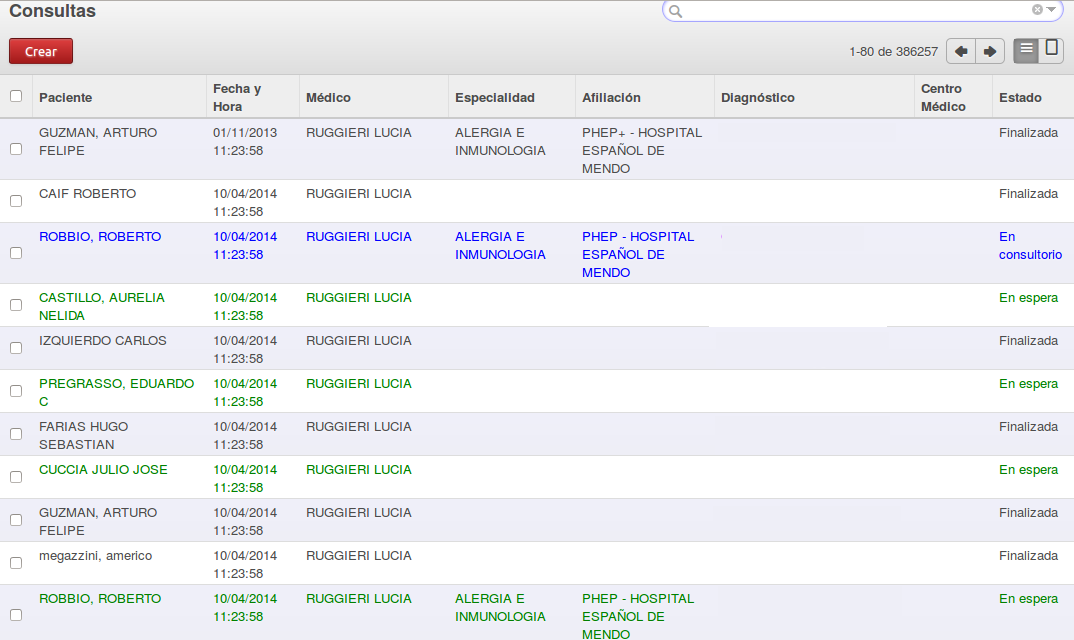
\includegraphics[width=.8\textwidth]{img/tp1/HE/HCUDConsulta}
      \caption{Listado de consultas médicas.}
      \label{consultas-auditor}
\end{correccionFigure}

{\correccionTexto
\subsubsection{Plantillas}
Muchas veces los médicos al elaborar pedidos médicos y dar indicaciones suelen repetir los detalles, para esto se desarrolló una funcionalidad para armar plantillas que al momento de cargar un los documentos mencionados antes lo pueden hacer automáticamente desde estas plantillas.\textbf{Figura \ref{plantilla}}
}

\begin{correccionFigure}[h]
      \centering
      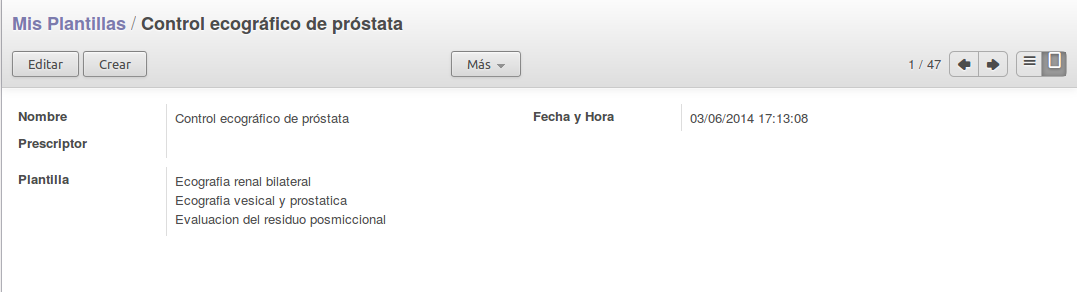
\includegraphics[width=.8\textwidth]{img/tp1/HE/PlantillaPM}
      \caption{Plantilla pedido médico}
      \label{plantilla}
\end{correccionFigure}

\section{Diagnóstico de la situación actual}
A continuación se presenta un modelo lógico integrando las funciones que prestan la aplicación antes relevada, haciendo hincapié en las interacciones de las mismas con los usuarios.


\subsection{Modelo lógico de la situación actual de Microsoft Health Vault}

El modelo lógico de Microsoft Health Vault, en su situación actual, se ilustra en la \textbf{Figura \ref{casoDeUsoHV}}.

\begin{correccionFigure} 
  \centering
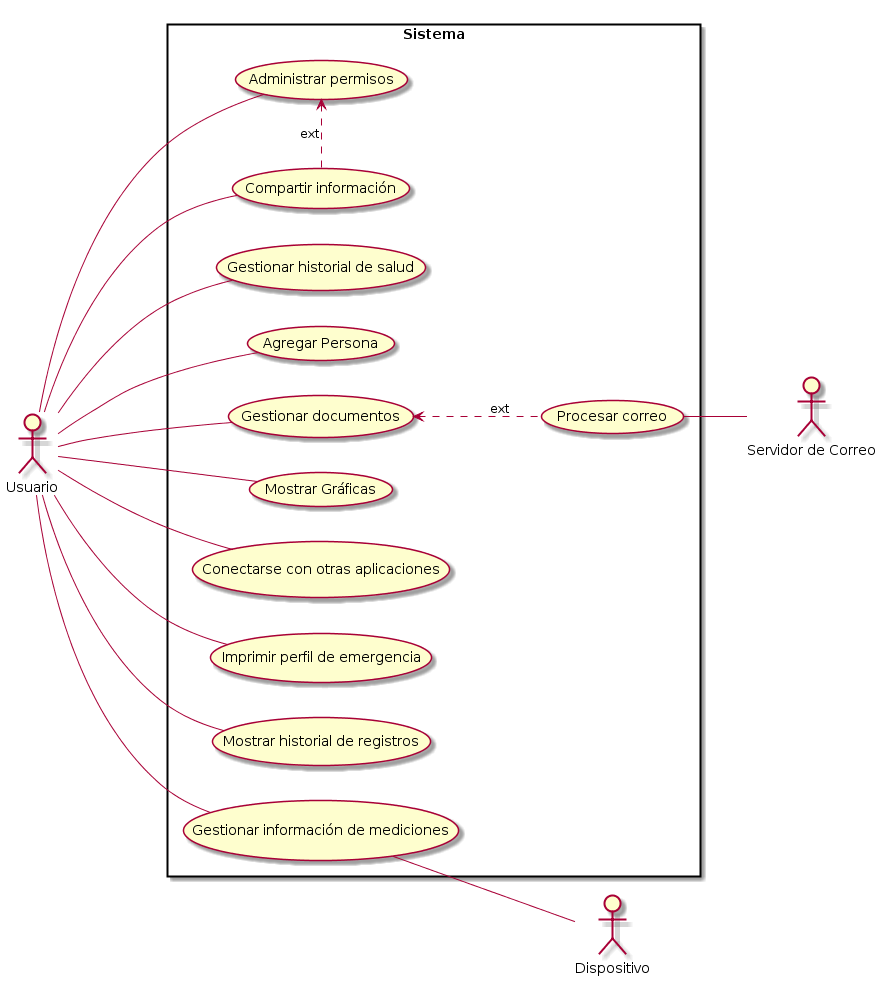
\includegraphics[width=1\textwidth]{img/tp1/cu-hv}
  \caption{Diagrama de Caso de Uso - Health Vault}
  \label{casoDeUsoHV}
\end{correccionFigure} 
 {\correccionTexto
\subsubsection{Agregar Persona}
Este caso de uso provee al usuario la posibilidad de crear una persona asociada a su cuenta(adicional a la persona por defecto que se crea cuando creamos la cuenta). Esto sucede cuando se cuenta con una persona a cargo a la que tenemos que gestionarle los registros médicos. Para crear esta nueva persona debemos proveerle un nombre,relación,fecha de nacimiento, país y provincia de nacimiento y sexo, entre otros atributos.
 
 \subsubsection{Compartir información}
El usuario debe establecer el destinatario al que se le enviará un correo con un link que le permita acceder a su perfil de emergencia y un código (autogenerado) que deberá ingresar en la web a la que será redireccionado. Ademas el usuario puede agregar una nota adicional adjunta al correo. De la misma manera podemos compartir mediciones y documentos.

\subsubsection{Administrar permisos}
El usuario debe poder decidir por cuanto tiempo una persona a la que se le dio acceso a su información podrá verla o editarla. Ademas debemos definir sobre que tipo de información queremos asignar o quitarle permisos.

\subsubsection{Conectarse con otras aplicaciones}
El usuario puede seleccionar entre distintas aplicaciones provistas por los repositorios del sistema operativo de su celular, para asesorarle en la gestión de su información personal, estos hacen uso de la API, que ofrece HealthVault para interactuar con el mismo.

\subsubsection{Gestionar historial de salud}
Consiste en añadir,editar y eliminar cierta información para la que no es necesaria su trazabilidad en el tiempo , de la cual un subconjunto formará parte del perfil de emergencia, como alergias,afecciones crónicas, suplementos y medicamentos actuales, contacto de emergencia y dispositivos médicos implantados.Y el resto de la información simplemente se guardará para ser reutilizado en otros formularios o por si el usuario necesita accederlo en el futuro, como citas,contactos,antecedentes familiares, resultados de laboratorio,seguros médicos, procedimiento, medicaciones e inmunizaciones.
 
\subsubsection{Gestionar información de mediciones}
Se le permite al usuario registrar sus mediciones(puede también,editar y eliminar) de aspectos relacionados a su salud personal como Peso, altura, Presión arterial, ejercicio, colesterol, composición, dimensión corporal, flujo máximo, menstruación, glucosa, comida y bebida. Es importante destacar que para estas mediciones es importante tener su evolución en el tiempo.

\subsubsection{Gestión de documentos}
	Este Caso de Uso, nos permite cargar archivos que contienen información referente a nuestra salud como imágenes, videos y radiografías. También nos permite guardar en nuestra cuenta, documentos XML que cumplen con la especificación CCR (Continuidad del registro del cuidado por sus siglas en inglés) y CCD, el primero es una especificación estándar de registros de salud la cual fue desarrollada dirigiendo los esfuerzos a satisfacer las necesidades de los profesionales de la salud por parte de un conglomerado de organizaciones ligadas a la salud. El segundo, está basada  en el primer documento, pero organizado en base a una estructura estandarizada llamada CDA (Arquitectura de documentos clínicos) establecida por un subconjunto de las organizaciones anteriores y el líder en estándares de la salud HL7. Ambos documentos permiten llevar un registro con información médica esencial de un paciente dado.
    
\subsubsection{Imprimir perfil de emergencia}
El usuario debe definir que tipo de perfil de emergencia desea imprimir , es decir, de bolsillo o completo,si desea un código de acceso web(que se generará automáticamente), y el nombre de la persona a la que está dirigido. Luego el sistema, en base al tipo de impresión solicitada, suprime o no algunos datos, y genera un PDF que contenga la información que considere de extrema importancia un profesional de salud.

\subsubsection{Mostrar gráficas}
Cuando el usuario ya tiene mediciones cargadas, se muestran a través de gráficas, así se puede evaluar su evolución en el tiempo, estas gráficas solo se aplican a las mediciones.

\subsubsection{Mostrar historial de registros}
Se le muestra al usuario una lista con todas las operaciones realizadas dentro de la plataforma, con un resumen de que se hizo en cada operación y que usuario,aplicación o dispositivo la realizó. Además el usuario puede acceder una vista en detalle y donde se muestra específicamente que información fue agregada, cambiada o eliminada.
}

\subsection{Modelo lógico de la situación actual de sistema de historia clínica}
El sistema de historia clínica del hospital español en su situación actual se ilustra en la \textbf{Figura \ref{mlogicoHCE}}.


\begin{figure}
  \centering
  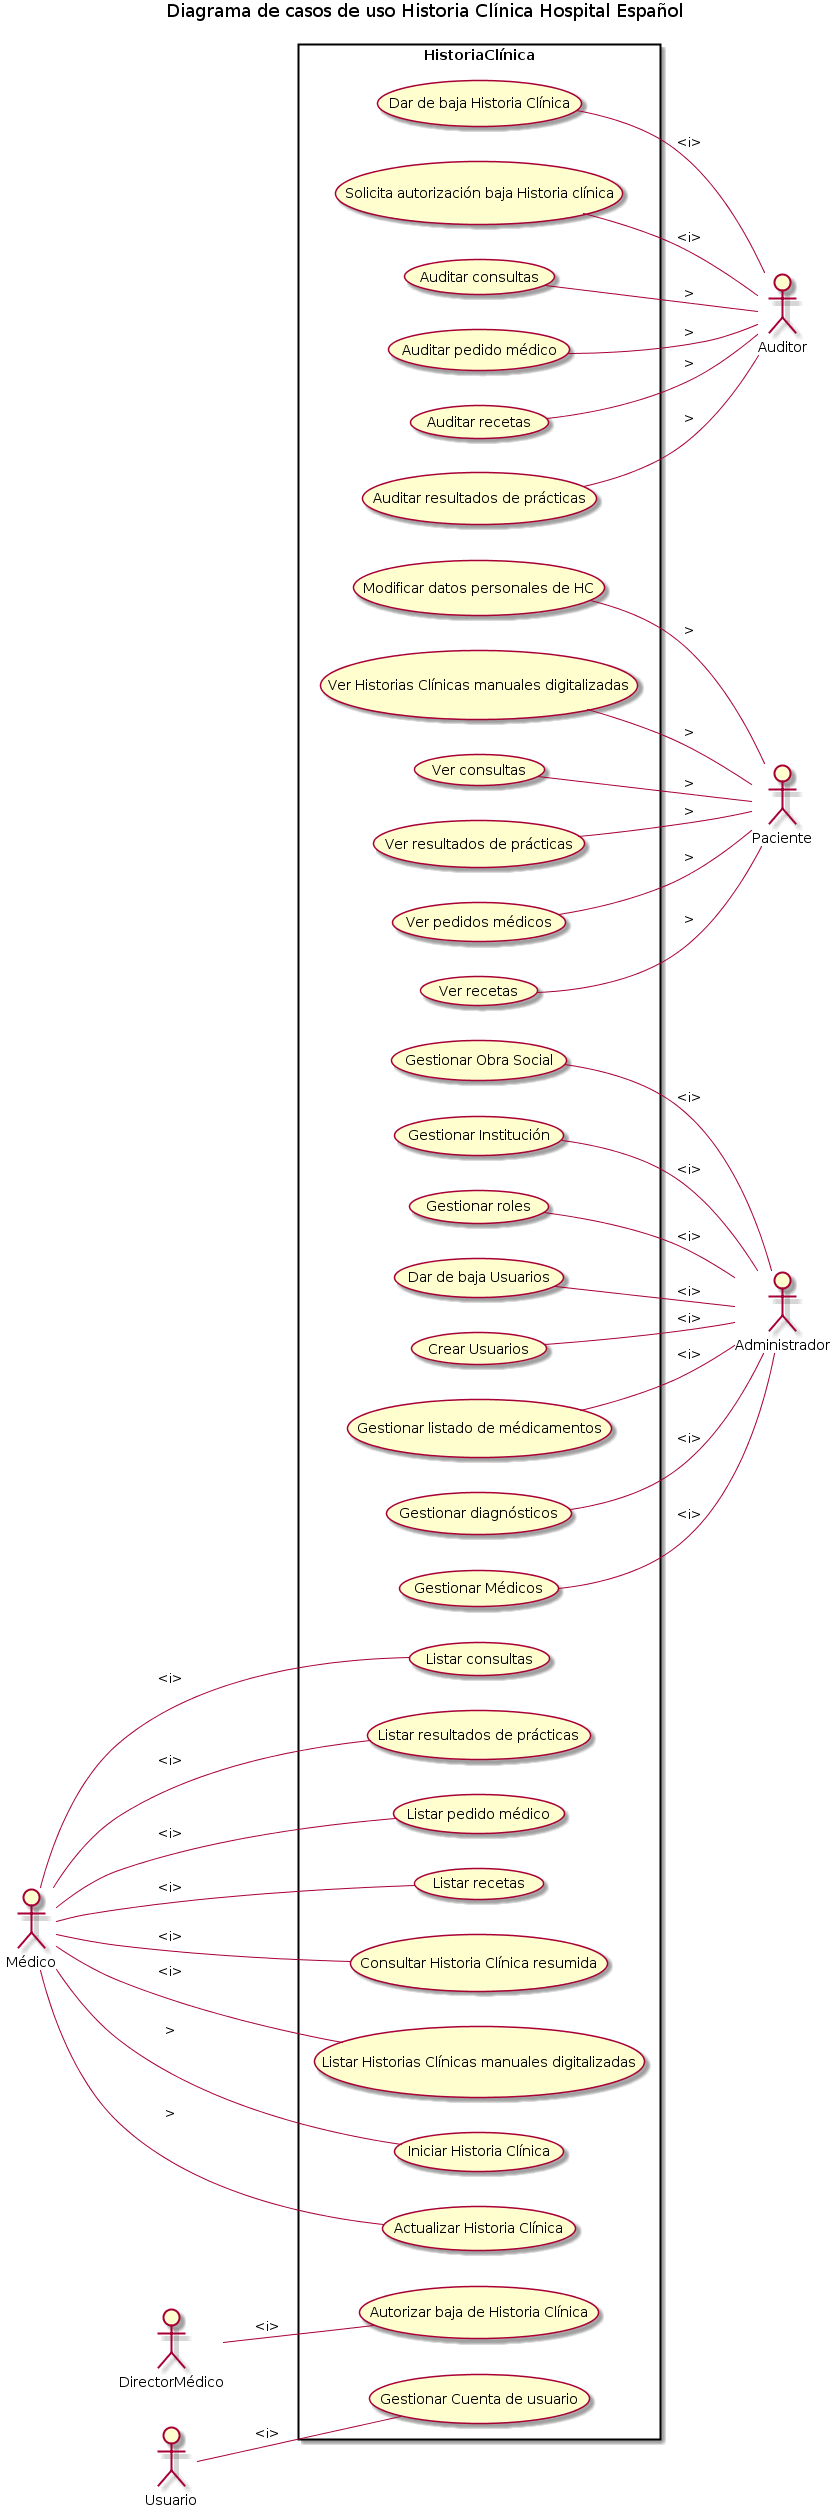
\includegraphics[width=.688\textwidth]{img/tp1/HCHEModeloFuncional}
  \caption{Modelo lógico - HCE}
  \label{mlogicoHCE}
\end{figure}


El corazón de todo sistema informático de la salud es el CDR. Éste se ilustra en la \textbf{Figura \ref{cdr}}.

\begin{figure}
  \centering
  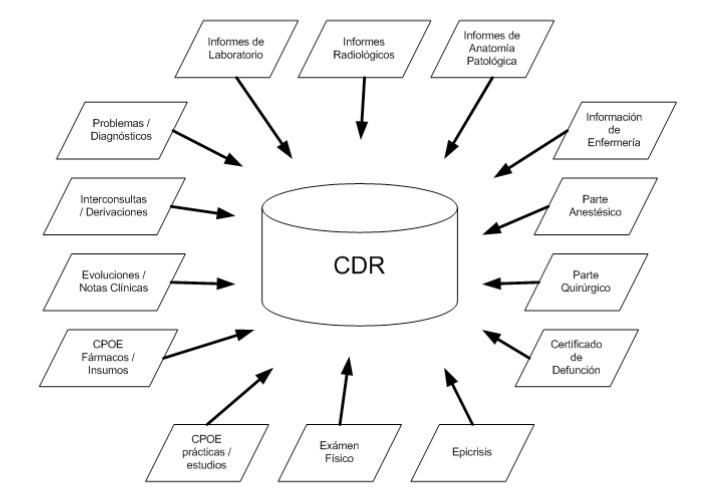
\includegraphics[width=.9\textwidth]{img/tp1/CDR}
  \caption{Clinical data repository - CDR} 
  \label{cdr}
\end{figure}

El CDR nutre de información a los distintos sistemas de salud. Esto se puede observar en la \textbf{Figura \ref{cdr-hce}}.
\begin{figure}
  \centering
  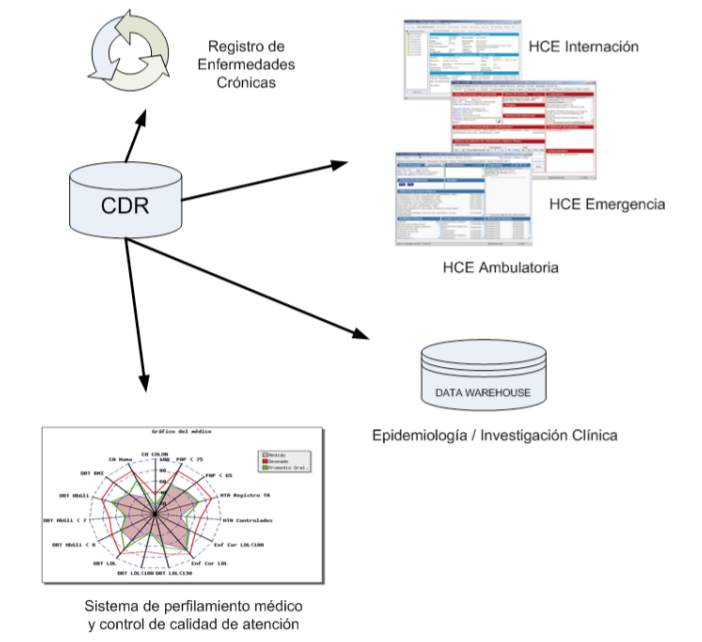
\includegraphics[width=.9\textwidth]{img/tp1/CDR-HCE}
  \caption{CDR - sistemas de salud} 
  \label{cdr-hce}
\end{figure}
\clearpage
\subsection{Problemas y necesidades detectadas}
Aquí se desarrollaran aquellos problemas y necesidades que se han detectado al realizar el análisis de los sistemas existentes en Argentina y en el mundo.
	\begin{itemize}

     \item No hemos encontrado una aplicación que proponga la gestión de documentos de salud personal y este disponible totalmente para Argentina.
     
     \item Los sistemas no proveen la posibilidad de adjuntar documentos a patologías, o relacionarlos entre si.
     
     \item No se provee una manera segura y directa por la que un laboratorio o un médico puedan solicitar información o enviarla promoviendo la organización eficaz de la misma. 
     
     \item Los sistemas actuales no ofrecen la posibilidad de recibir una devolución o comentarios del médico sobre información o documentación compartida.

% No hay libre disposicion de los documentos

%     \item No hay sistemas donde se haga un seguimiento completo de las embarazadas que incluya información previa al embarazo y un seguimiento posterior sobre el niño naciente. Lo consideramos muy importante ya que los acontecimientos durante la gestación del niño pueden afectarle en un futuro.
     


\end{itemize}

\clearpage
\subsection{Objetivos y alcances preliminares del nuevo sistema}

Los objetivos del proyecto fueron realizados teniendo en cuenta la misión que se detalla a continuación:

\begin{quote}
\small \textit{ "Brindarle una mayor cantidad de datos al profesional de salud, mejorando el proceso y resultados de sus conclusiones, para así ofrecer mejor calidad de vida a los usuarios de nuestro sistema."}
 \end{quote}
 \begin{comment}


 De aquí se desprenden
     \begin{itemize}
		\item Brindar al profesional de salud datos históricos del paciente.
        \item Permitir  al usuario poder gestionar todos sus análisis y mediciones relacionadas a la salud.
        \item Mejorar el procesos de atención al paciente %Disminuir las visitas al médico en un 25%
        \item Brindar una aplicación integradora de la información de salud.
        \item Mejorar la ca
    \end{itemize}
\end{comment}

{\correccionTexto
\subsubsection{Objetivos generales para el 2015}  
%	\item Permitir al usuario la gestión y el acceso privado y total a sus datos de estudios clínicos e información médica, promoviendo la independencia del usuario con respecto a los institutos de salud.
\begin{comment}
		\item Permitir a los usuarios del sistema añadir todo tipo de mediciones referidos a su salud. 
	    \item Permitir a los usuarios del sistema añadir todo tipo de análisis clínicos.
	    \item Permitir a los usuarios del sistema añadir información relacionada a visitas al medico, vacunación y diagnósticos.
	    \item Permitir a los usuarios tener acceso único y privado a su información, brindándole la posibilidad de asignar permisos CRUD (Create, Read, Update, Delete) a otros usuarios.
	    \item Permitir a los usuarios generar vistas de su información a lo largo del tiempo, a través de gráficas , tablas y resúmenes.
    	\item Permitir realizar comentarios, a usuarios autorizados, sobre información compartida.
	    \item Ofrecer avisos y recomendaciones relacionados a la salud del paciente.
        %%%%%%%%%%%%%%%%%%%%%%%%%%%%%%%%%%%%%%%%%%%%%%%%%%%%%%%%%%%%%%
        %\item alcanzar una cantidad de usuarios
    %\item cubrir una determinada cantidad de reamas de la medicina
    %\item Objetivos RME (sobre datos clínicos):
    %\begin{itemize}
	%	\item Adquisición
    %    \item Almacenamiento
    %    \item Recuperacion
    %    \item Procesamiento
    %    \item Intercambio
	%\end{itemize}
    
    %\item específico, sobre que sistemas vamos a recibir información
    %\item Permitir al usuario la gestión y el acceso privado y total a sus datos de estudios clínicos e información médica para brindarle una mejor atención médica.
    %\item Permitir a los profesionales médicos el acceso a información compartida para mejorar el proceso de seguimiento y control.
	%\item Brindar recomendaciones de salud a partir de la información recopilada.        
\end{comment}


    \begin{itemize}
	    \item Brindarle al usuario la posibilidad de acceder a la totalidad de sus análisis a través de su cuenta de Salud.
    	\item Cambiar el paradigma de atención médica, logrando aumentar en un 50\% las consultas vía on-line.
        \item Brindar un sistema integrador que le permita al usuario cambiar de médico u hospital cuando el lo desee sin perder información.
	\end{itemize}
	}



\subsection{Funciones y alcances preliminares}
Las funciones y alcances que se definieron se fundamentan en los user story. Un user story describe una funcionalidad que, por si misma aporta valor al usuario.

	\begin{itemize}           
    %%%
	\item Como paciente, quiero  añadir al sistema mis estudios realizados para evitar posibles perdidas.
    
    Alcance: se desarrollará el modulo de carga de estudios permitiendo la carga de todo tipo de archivos.
    %Aclaramos, que nos referimos a imágenes,  o archivos especificos ? 
	%\item Como paciente quiero cargar los estudios a partir de una foto para agilizar el proceso de carga.
    % se separó en dos user estorbes
	\item Como paciente, quiero  añadir información de mi perfil de salud o mediciones regulares para que el médico cuente con más y mejor información al momento de realizar el diagnóstico.
    
    Alcance: se permitirá la carga del peso, dimensiones corporales, medición de glucosa, colesterol y presión arterial. 
    Además permitiremos registrar información que complete el perfil del paciente como alergias,afecciones crónicas, suplementos y medicamentos, artefactos médicos e incidencias que considere importante.
	%%%
	\item Como paciente, quiero que los sistemas de salud existentes puedan cargar sus resultados directamente en mi carpeta de salud para centralizar mi información.
    
    Alcance: se ofrecerá una API de acceso para la carga y lectura de información por parte de agentes externos a nuestro sistema y le permitiremos al paciente gestionar los correspondientes permisos para esto.
    
	%\item Como paciente quiero dar acceso a un laboratorio para que cargue información para evitar tener q ir al laboratorio.
    %
	\item Como paciente, quiero asociar un dispositivo para agilizar y ampliar la carga de datos.
    
   Alcance: se ofrecerá una API de acceso para la carga y lectura de información por parte de agentes externos a nuestro sistema, esto permitirá integrar dispositivos ya existentes en el mercado y facilitará la adopción del sistema por parte de personas que ya cuenten con los mismos.
  %%%
	\item Como paciente, quiero categorizar mis estudios por rama de medicina, para lograr una mejor organización y navegabilidad en el sistema.
    
    Alcance: Se solicitará una clasificación de la documentación a través de ciertas ramas definidas por defecto en el sistema y permitiremos el uso de ``tags'' personalizados.
     %%%
	\item Como laboratorio, quiero cargar información de un paciente en su cuenta para ahorrarle las molestias de volver.
    
   Alcance: se ofrecerá una API de acceso para la carga y lectura de información por parte de agentes externos a nuestro sistema, además de una interfaz de carga web y para dispositivos móviles.
    %%%
    \item Como paciente, quiero guardar mi información de manera local para tener un respaldo.
    
    Alcance: se permitirá la exportación de todos los documentos.
    % abría que aclarar que puede ser exportarlo a la DB local y en forma física (imrpimir)
    % Como paciente quiero guardar mi información en forma privada localmente para que solo yo la pueda ver
    %%%
	\item Como paciente, quiero agregar personas a mi grupo familiar para llevar el seguimiento de los mismos.
    
    Alcance: se permitirá la creación de cuentas asociadas a otras y su gestión de permisos.
    %%%
	\item Como paciente, quiero modificar los permisos de visualización de mis datos con respecto a  cada uno de los integrantes de grupo familiar para tener un control total sobre mi privacidad.
    
    Alcance: Se permitirá la gestión total de los permisos de acceso a la información propia.
    %%%
	\item Como paciente quiero que no sea necesario ir al hospital para que un medico me comunique los resultados del análisis.
    
    Alcance: Se ofrecerá un medio de comunicación seguro y privado con el médico ademas de permitir realizar comentarios por parte del profesional sobre documentación compartida.
    
    %\item Como paciente quiero compartir información personal con médicos para brindarle información útil sobre mi estado de salud.
    %\item Como paciente quiero elegir que información subir al sistema compartido para que solo cierta información este compartida en la nube
    %Alcance: Se permitirá al paciente elegir o ingresar, uno o más médicos con el que compartirá la información  previamente seleccionada. 
    %%%
	\item Como usuario quiero registrarme con una cuenta de Facebook y/o Google para facilitar la inscripción al sitio y el manejo de credenciales.
    
    Alcance: Se desarrollará el modulo de autenticación y registración utilizando una cuenta de Facebook o Google.
%	\item Como paciente quiero elegir que información subir al sistema para que solo cierta información este compartida.
    %%%
 	\item Como mujer embarazada quiero llevar la información de mi hijo para transmitírsela cuando nazca.
    
    Alcance: Se desarrollará el módulo de creación de cuentas asociadas donde se podrá dejar información compartida para la cuenta del hijo.
    
   %%%    
    \item Como médico quiero ver gráficas que resuman la información de un paciente para poder ver sus cambios a lo largo de la historia y así apoyar la toma de decisiones y el diagnóstico.
    
    Alcance: Se desarrollará el modulo de visualización de datos que consiste en presentar la información pertinente, de un período de tiempo, de diferentes maneras, ya sea tanto en formato de tablas como de gráficos. 
  %%%
	\item Como paciente, quiero acceder a mis documentos desde cualquier lugar para hacer uso de ellos cuando los necesite.
    
    Alcance: Se permitirá el acceso a la información del paciente a través de una cuenta privada que podrá acceder desde plataformas web o teléfonos móviles. % con acceso a internet o no, en el caso en que posea los datos almacenado localmente.
    
	%%%
	\item Como paciente quiero ver gráficas que resuman mi información en particular para poder ver mis cambios a lo largo de la historia.
    
    Alcance: Se desarrollará el modulo de visualización de datos que consiste en presentar la información pertinente, de un período de tiempo, de diferentes maneras, ya sea tanto en formato de tablas como de gráficos. 
    %%%
	\item Como paciente quiero obtener un resumen de mi información de salud básica para hacer uso de la misma en caso de una emergencia.
    
    Alcance: Se permitirá obtener un perfil personal para los casos de emergencia que cuente con la siguiente información: afecciones crónicas, suplementos, medicamento y artefactos médicos
	%%%
	\item Como paciente quiero ver en un único lugar los comentarios realizados por los médicos autorizados para una lectura rápida.
    
    Alcance: Se realizará una sección de comentarios que permitirá al paciente ver todos los comentarios realizados por el médico en cada una de las especialidades que el seleccione.
    
%	\item Como paciente quiero recibir recomendaciones sobre los estudios comunes y su periodicidad que suelen realizar las personas para mejorar mi calidad de vida.
    

%	\item Como médico quiero comentar estudios de un paciente para tener una forma de comunicación directa con el paciente.
%\item Como médico quiero visualizar la información de un paciente para apoyar la toma de decisiones y el diagnóstico.  
    %%%
	\item Como médico quiero verificar que las personas que solicitan mi atención sean pacientes para mantener mi cantidad de consultas en una cantidad controlable.
    
    Alcance: el médico podrá aceptar o no, a personas como sus pacientes antes de recibir información de los mismos o solicitudes.
    %%%
	\item Como médico quiero diagnosticar a un paciente, para darle un cierre a una incidencia planteada por la persona.
    
    Alcance: Se permitirá la interacción a través de mensajes con el paciente y comentarios sobre incidencias.
	
   % \item Como paciente quiero recibir recomendaciones sobre vacunaciones y practicas medicas de acuerdo a situaciones externas que exceden mis conocimientos para afrontar estos cambios.
    \item Como paciente quiero recibir noticias, recomendaciones de otros usuarios o información de interés para informarme o notificarme sobre una afección o alguna cuestión de salud.
    
    Alcance: no se llevará a cabo esta funcionalidad en el año actual. % No se dará soporte
    
	%\item Como paciente, quiero obtener información y enlaces útiles sobre enfermedades para capacitarme.
	\item Como paciente quiero obtener notificaciones y avisos de sucesos importantes para estar preparado ante circunstancias.
    
    Alcance: no se llevará a cabo esta funcionalidad en el año actual. % No se dará soporte porque implica evaluar información para determinar cuando esta alto el nivel de algún indicador,  e implicaría extender los tiempos
    
\end{itemize}
